\documentclass[1p]{elsarticle_modified}
%\bibliographystyle{elsarticle-num}

%\usepackage[colorlinks]{hyperref}
%\usepackage{abbrmath_seonhwa} %\Abb, \Ascr, \Acal ,\Abf, \Afrak
\usepackage{amsfonts}
\usepackage{amssymb}
\usepackage{amsmath}
\usepackage{amsthm}
\usepackage{scalefnt}
\usepackage{amsbsy}
\usepackage{kotex}
\usepackage{caption}
\usepackage{subfig}
\usepackage{color}
\usepackage{graphicx}
\usepackage{xcolor} %% white, black, red, green, blue, cyan, magenta, yellow
\usepackage{float}
\usepackage{setspace}
\usepackage{hyperref}

\usepackage{tikz}
\usetikzlibrary{arrows}

\usepackage{multirow}
\usepackage{array} % fixed length table
\usepackage{hhline}

%%%%%%%%%%%%%%%%%%%%%
\makeatletter
\renewcommand*\env@matrix[1][\arraystretch]{%
	\edef\arraystretch{#1}%
	\hskip -\arraycolsep
	\let\@ifnextchar\new@ifnextchar
	\array{*\c@MaxMatrixCols c}}
\makeatother %https://tex.stackexchange.com/questions/14071/how-can-i-increase-the-line-spacing-in-a-matrix
%%%%%%%%%%%%%%%

\usepackage[normalem]{ulem}

\newcommand{\msout}[1]{\ifmmode\text{\sout{\ensuremath{#1}}}\else\sout{#1}\fi}
%SOURCE: \msout is \stkout macro in https://tex.stackexchange.com/questions/20609/strikeout-in-math-mode

\newcommand{\cancel}[1]{
	\ifmmode
	{\color{red}\msout{#1}}
	\else
	{\color{red}\sout{#1}}
	\fi
}

\newcommand{\add}[1]{
	{\color{blue}\uwave{#1}}
}

\newcommand{\replace}[2]{
	\ifmmode
	{\color{red}\msout{#1}}{\color{blue}\uwave{#2}}
	\else
	{\color{red}\sout{#1}}{\color{blue}\uwave{#2}}
	\fi
}

\newcommand{\Sol}{\mathcal{S}} %segment
\newcommand{\D}{D} %diagram
\newcommand{\A}{\mathcal{A}} %arc


%%%%%%%%%%%%%%%%%%%%%%%%%%%%%5 test

\def\sl{\operatorname{\textup{SL}}(2,\Cbb)}
\def\psl{\operatorname{\textup{PSL}}(2,\Cbb)}
\def\quan{\mkern 1mu \triangleright \mkern 1mu}

\theoremstyle{definition}
\newtheorem{thm}{Theorem}[section]
\newtheorem{prop}[thm]{Proposition}
\newtheorem{lem}[thm]{Lemma}
\newtheorem{ques}[thm]{Question}
\newtheorem{cor}[thm]{Corollary}
\newtheorem{defn}[thm]{Definition}
\newtheorem{exam}[thm]{Example}
\newtheorem{rmk}[thm]{Remark}
\newtheorem{alg}[thm]{Algorithm}

\newcommand{\I}{\sqrt{-1}}
\begin{document}

%\begin{frontmatter}
%
%\title{Boundary parabolic representations of knots up to 8 crossings}
%
%%% Group authors per affiliation:
%\author{Yunhi Cho} 
%\address{Department of Mathematics, University of Seoul, Seoul, Korea}
%\ead{yhcho@uos.ac.kr}
%
%
%\author{Seonhwa Kim} %\fnref{s_kim}}
%\address{Center for Geometry and Physics, Institute for Basic Science, Pohang, 37673, Korea}
%\ead{ryeona17@ibs.re.kr}
%
%\author{Hyuk Kim}
%\address{Department of Mathematical Sciences, Seoul National University, Seoul 08826, Korea}
%\ead{hyukkim@snu.ac.kr}
%
%\author{Seokbeom Yoon}
%\address{Department of Mathematical Sciences, Seoul National University, Seoul, 08826,  Korea}
%\ead{sbyoon15@snu.ac.kr}
%
%\begin{abstract}
%We find all boundary parabolic representation of knots up to 8 crossings.
%
%\end{abstract}
%\begin{keyword}
%    \MSC[2010] 57M25 
%\end{keyword}
%
%\end{frontmatter}

%\linenumbers
%\tableofcontents
%
\newcommand\colored[1]{\textcolor{white}{\rule[-0.35ex]{0.8em}{1.4ex}}\kern-0.8em\color{red} #1}%
%\newcommand\colored[1]{\textcolor{white}{ #1}\kern-2.17ex	\textcolor{white}{ #1}\kern-1.81ex	\textcolor{white}{ #1}\kern-2.15ex\color{red}#1	}

{\Large $\underline{12a_{0164}~(K12a_{0164})}$}

\setlength{\tabcolsep}{10pt}
\renewcommand{\arraystretch}{1.6}
\vspace{1cm}\begin{tabular}{m{100pt}>{\centering\arraybackslash}m{274pt}}
\multirow{5}{120pt}{
	\centering
	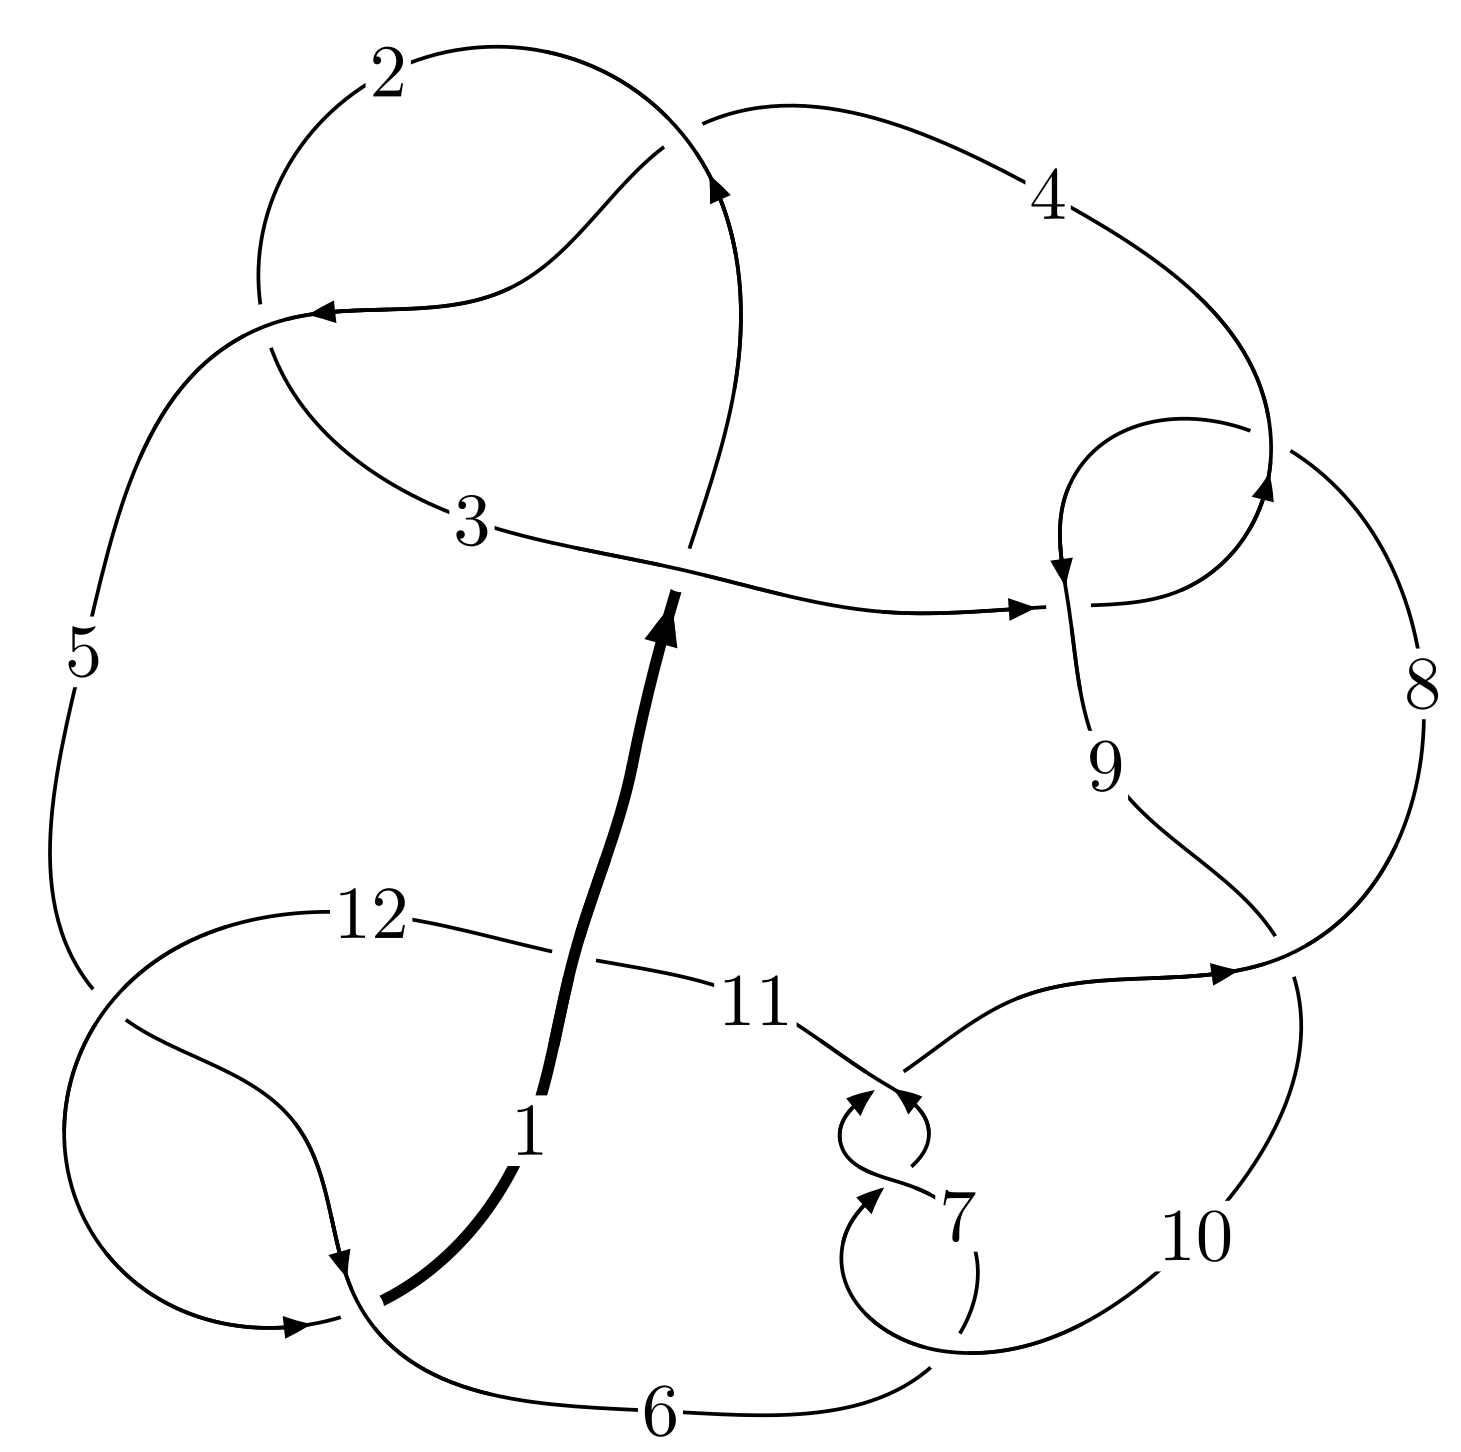
\includegraphics[width=112pt]{../../../GIT/diagram.site/Diagrams/png/965_12a_0164.png}\\
\ \ \ A knot diagram\footnotemark}&
\allowdisplaybreaks
\textbf{Linearized knot diagam} \\
\cline{2-2}
 &
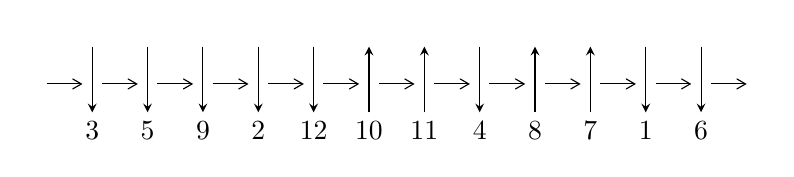
\begin{tikzpicture}[x=20pt, y=17pt]
	% nodes
	\node (C0) at (0, 0) {};
	\node (C1) at (1, 0) {};
	\node (C1U) at (1, +1) {};
	\node (C1D) at (1, -1) {3};

	\node (C2) at (2, 0) {};
	\node (C2U) at (2, +1) {};
	\node (C2D) at (2, -1) {5};

	\node (C3) at (3, 0) {};
	\node (C3U) at (3, +1) {};
	\node (C3D) at (3, -1) {9};

	\node (C4) at (4, 0) {};
	\node (C4U) at (4, +1) {};
	\node (C4D) at (4, -1) {2};

	\node (C5) at (5, 0) {};
	\node (C5U) at (5, +1) {};
	\node (C5D) at (5, -1) {12};

	\node (C6) at (6, 0) {};
	\node (C6U) at (6, +1) {};
	\node (C6D) at (6, -1) {10};

	\node (C7) at (7, 0) {};
	\node (C7U) at (7, +1) {};
	\node (C7D) at (7, -1) {11};

	\node (C8) at (8, 0) {};
	\node (C8U) at (8, +1) {};
	\node (C8D) at (8, -1) {4};

	\node (C9) at (9, 0) {};
	\node (C9U) at (9, +1) {};
	\node (C9D) at (9, -1) {8};

	\node (C10) at (10, 0) {};
	\node (C10U) at (10, +1) {};
	\node (C10D) at (10, -1) {7};

	\node (C11) at (11, 0) {};
	\node (C11U) at (11, +1) {};
	\node (C11D) at (11, -1) {1};

	\node (C12) at (12, 0) {};
	\node (C12U) at (12, +1) {};
	\node (C12D) at (12, -1) {6};
	\node (C13) at (13, 0) {};

	% arrows
	\draw[->,>={angle 60}]
	(C0) edge (C1) (C1) edge (C2) (C2) edge (C3) (C3) edge (C4) (C4) edge (C5) (C5) edge (C6) (C6) edge (C7) (C7) edge (C8) (C8) edge (C9) (C9) edge (C10) (C10) edge (C11) (C11) edge (C12) (C12) edge (C13) ;	\draw[->,>=stealth]
	(C1U) edge (C1D) (C2U) edge (C2D) (C3U) edge (C3D) (C4U) edge (C4D) (C5U) edge (C5D) (C6D) edge (C6U) (C7D) edge (C7U) (C8U) edge (C8D) (C9D) edge (C9U) (C10D) edge (C10U) (C11U) edge (C11D) (C12U) edge (C12D) ;
	\end{tikzpicture} \\
\hhline{~~} \\& 
\textbf{Solving Sequence} \\ \cline{2-2} 
 &
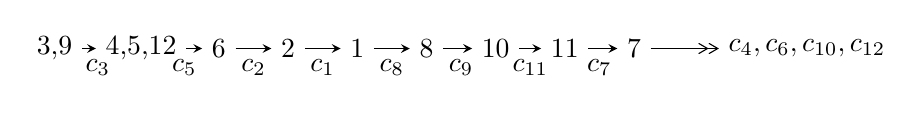
\begin{tikzpicture}[x=25pt, y=7pt]
	% node
	\node (A0) at (-1/8, 0) {3,9};
	\node (A1) at (9/8, 0) {4,5,12};
	\node (A2) at (9/4, 0) {6};
	\node (A3) at (13/4, 0) {2};
	\node (A4) at (17/4, 0) {1};
	\node (A5) at (21/4, 0) {8};
	\node (A6) at (25/4, 0) {10};
	\node (A7) at (29/4, 0) {11};
	\node (A8) at (33/4, 0) {7};
	\node (C1) at (1/2, -1) {$c_{3}$};
	\node (C2) at (7/4, -1) {$c_{5}$};
	\node (C3) at (11/4, -1) {$c_{2}$};
	\node (C4) at (15/4, -1) {$c_{1}$};
	\node (C5) at (19/4, -1) {$c_{8}$};
	\node (C6) at (23/4, -1) {$c_{9}$};
	\node (C7) at (27/4, -1) {$c_{11}$};
	\node (C8) at (31/4, -1) {$c_{7}$};
	\node (A9) at (43/4, 0) {$c_{4},c_{6},c_{10},c_{12}$};

	% edge
	\draw[->,>=stealth]	
	(A0) edge (A1) (A1) edge (A2) (A2) edge (A3) (A3) edge (A4) (A4) edge (A5) (A5) edge (A6) (A6) edge (A7) (A7) edge (A8) ;
	\draw[->>,>={angle 60}]	
	(A8) edge (A9);
\end{tikzpicture} \\ 

\end{tabular} \\

\footnotetext{
The image of knot diagram is generated by the software ``\textbf{Draw programme}" developed by Andrew Bartholomew(\url{http://www.layer8.co.uk/maths/draw/index.htm\#Running-draw}), where we modified some parts for our purpose(\url{https://github.com/CATsTAILs/LinksPainter}).
}\phantom \\ \newline 
\centering \textbf{Ideals for irreducible components\footnotemark of $X_{\text{par}}$} 
 
\begin{align*}
I^u_{1}&=\langle 
798299739247 u^{24}+2218887488039 u^{23}+\cdots+14116099211116 d-8843381349140,\\
\phantom{I^u_{1}}&\phantom{= \langle  }-364885635753 u^{24}+1117648334550 u^{23}+\cdots+28232198422232 c-44559223365168,\\
\phantom{I^u_{1}}&\phantom{= \langle  }458802669672 u^{24}+367351897733 u^{23}+\cdots+7058049605558 b-1244576019090,\\
\phantom{I^u_{1}}&\phantom{= \langle  }-1687329917173 u^{24}-1804551705088 u^{23}+\cdots+28232198422232 a-30643572770096,\\
\phantom{I^u_{1}}&\phantom{= \langle  }u^{25}+2 u^{24}+\cdots-16 u-8\rangle \\
I^u_{2}&=\langle 
d+1,\;2 u^{10} a+u^{10}+\cdots-4 a+4,\;- u^{10} a+u^{10}+\cdots+b-2,\;-3 u^{10} a+u^{10}+\cdots+2 a^2-2 a,\\
\phantom{I^u_{2}}&\phantom{= \langle  }u^{11}-3 u^{10}+6 u^9-7 u^8+7 u^7-3 u^6-2 u^5+8 u^4-7 u^3+5 u^2-2 u+2\rangle \\
I^u_{3}&=\langle 
d+1,\;- u^7 a-3 u^5 a+u^5-2 u^3 a-3 a u+c+a+u,\;- u^7 a+u^7+u^5- u^3 a+2 u^3+b+u-1,\\
\phantom{I^u_{3}}&\phantom{= \langle  }2 u^8 a-2 u^8+\cdots+2 a-2,\;u^9+u^8+2 u^7+u^6+3 u^5+u^4+2 u^3+u-1\rangle \\
I^u_{4}&=\langle 
d+1,\;2 u^7 c- u^8+2 u^6 c+2 u^5 c- u^6+2 u^4 c+u^5+4 u^3 c-2 u^4+2 u^2 c+c^2- u^2+c+2 u,\\
\phantom{I^u_{4}}&\phantom{= \langle  }- u^7- u^5-2 u^3+b- u,\;- u^5+a- u,\;u^9+u^8+2 u^7+u^6+3 u^5+u^4+2 u^3+u-1\rangle \\
I^u_{5}&=\langle 
2 u^8+2 u^7+4 u^6+4 u^5+6 u^4+4 u^3+4 u^2+d+4 u,\;2 u^8+2 u^6+4 u^4+2 u^2+c+1,\;- u^7- u^5-2 u^3+b- u,\\
\phantom{I^u_{5}}&\phantom{= \langle  }- u^5+a- u,\;u^9+u^8+2 u^7+u^6+3 u^5+u^4+2 u^3+u-1\rangle \\
\\
I^v_{1}&=\langle 
a,\;d+1,\;c+a+1,\;b-1,\;v+1\rangle \\
I^v_{2}&=\langle 
c,\;d+1,\;b,\;a-1,\;v-1\rangle \\
I^v_{3}&=\langle 
a,\;d+1,\;c+a,\;b-1,\;v-1\rangle \\
I^v_{4}&=\langle 
a,\;d a- c-1,\;d v+v-1,\;c v+a v- a+v,\;b-1\rangle \\
\end{align*}
\raggedright * 8 irreducible components of $\dim_{\mathbb{C}}=0$, with total 95 representations.\\
\raggedright * 1 irreducible components of $\dim_{\mathbb{C}}=1$ \\
\footnotetext{All coefficients of polynomials are rational numbers. But the coefficients are sometimes approximated in decimal forms when there is not enough margin.}
\newpage
\renewcommand{\arraystretch}{1}
\centering \section*{I. $I^u_{1}= \langle 7.98\times10^{11} u^{24}+2.22\times10^{12} u^{23}+\cdots+1.41\times10^{13} d-8.84\times10^{12},\;-3.65\times10^{11} u^{24}+1.12\times10^{12} u^{23}+\cdots+2.82\times10^{13} c-4.46\times10^{13},\;4.59\times10^{11} u^{24}+3.67\times10^{11} u^{23}+\cdots+7.06\times10^{12} b-1.24\times10^{12},\;-1.69\times10^{12} u^{24}-1.80\times10^{12} u^{23}+\cdots+2.82\times10^{13} a-3.06\times10^{13},\;u^{25}+2 u^{24}+\cdots-16 u-8 \rangle$}
\flushleft \textbf{(i) Arc colorings}\\
\begin{tabular}{m{7pt} m{180pt} m{7pt} m{180pt} }
\flushright $a_{3}=$&$\begin{pmatrix}1\\0\end{pmatrix}$ \\
\flushright $a_{9}=$&$\begin{pmatrix}0\\u\end{pmatrix}$ \\
\flushright $a_{4}=$&$\begin{pmatrix}1\\u^2\end{pmatrix}$ \\
\flushright $a_{5}=$&$\begin{pmatrix}0.0597662 u^{24}+0.0639182 u^{23}+\cdots-0.107083 u+1.08541\\-0.0650042 u^{24}-0.0520472 u^{23}+\cdots+0.578878 u+0.176334\end{pmatrix}$ \\
\flushright $a_{12}=$&$\begin{pmatrix}0.0129244 u^{24}-0.0395877 u^{23}+\cdots+0.145173 u+1.57831\\-0.0565524 u^{24}-0.157188 u^{23}+\cdots-1.05131 u+0.626475\end{pmatrix}$ \\
\flushright $a_{6}=$&$\begin{pmatrix}0.0747149 u^{24}+0.105730 u^{23}+\cdots+0.724685 u+0.690091\\0.00202430 u^{24}+0.0813992 u^{23}+\cdots+0.686595 u-0.973634\end{pmatrix}$ \\
\flushright $a_{2}=$&$\begin{pmatrix}0.0597662 u^{24}+0.0639182 u^{23}+\cdots-0.107083 u+1.08541\\0.0375166 u^{24}+0.0396045 u^{23}+\cdots-0.990575 u-0.621247\end{pmatrix}$ \\
\flushright $a_{1}=$&$\begin{pmatrix}0.0972828 u^{24}+0.103523 u^{23}+\cdots-1.09766 u+0.464165\\0.0375166 u^{24}+0.0396045 u^{23}+\cdots-0.990575 u-0.621247\end{pmatrix}$ \\
\flushright $a_{8}=$&$\begin{pmatrix}u\\u^3+u\end{pmatrix}$ \\
\flushright $a_{10}=$&$\begin{pmatrix}u^3\\u^5+u^3+u\end{pmatrix}$ \\
\flushright $a_{11}=$&$\begin{pmatrix}0.0159383 u^{24}-0.0332769 u^{23}+\cdots-0.0633916 u+1.31412\\-0.0587766 u^{24}-0.139007 u^{23}+\cdots-0.788077 u+0.624033\end{pmatrix}$ \\
\flushright $a_{7}=$&$\begin{pmatrix}0.0395277 u^{24}+0.0675081 u^{23}+\cdots+0.598270 u+0.845409\\-0.0839809 u^{24}-0.0749523 u^{23}+\cdots+1.66833 u+0.315163\end{pmatrix}$\\&\end{tabular}
\flushleft \textbf{(ii) Obstruction class $= -1$}\\~\\
\flushleft \textbf{(iii) Cusp Shapes $= \frac{8058725701665}{7058049605558} u^{24}+\frac{10736954342885}{7058049605558} u^{23}+\cdots-\frac{38478403451674}{3529024802779} u-\frac{29622418287164}{3529024802779}$}\\~\\
\newpage\renewcommand{\arraystretch}{1}
\flushleft \textbf{(iv) u-Polynomials at the component}\newline \\
\begin{tabular}{m{50pt}|m{274pt}}
Crossings & \hspace{64pt}u-Polynomials at each crossing \\
\hline $$\begin{aligned}c_{1},c_{11}\end{aligned}$$&$\begin{aligned}
&u^{25}+12 u^{24}+\cdots+3 u+1
\end{aligned}$\\
\hline $$\begin{aligned}c_{2},c_{4},c_{5}\\c_{12}\end{aligned}$$&$\begin{aligned}
&u^{25}-2 u^{24}+\cdots- u+1
\end{aligned}$\\
\hline $$\begin{aligned}c_{3},c_{8}\end{aligned}$$&$\begin{aligned}
&u^{25}-2 u^{24}+\cdots-16 u+8
\end{aligned}$\\
\hline $$\begin{aligned}c_{6},c_{7},c_{10}\end{aligned}$$&$\begin{aligned}
&u^{25}+2 u^{24}+\cdots+8 u+4
\end{aligned}$\\
\hline $$\begin{aligned}c_{9}\end{aligned}$$&$\begin{aligned}
&u^{25}-6 u^{24}+\cdots+64 u+64
\end{aligned}$\\
\hline
\end{tabular}\\~\\
\newpage\renewcommand{\arraystretch}{1}
\flushleft \textbf{(v) Riley Polynomials at the component}\newline \\
\begin{tabular}{m{50pt}|m{274pt}}
Crossings & \hspace{64pt}Riley Polynomials at each crossing \\
\hline $$\begin{aligned}c_{1},c_{11}\end{aligned}$$&$\begin{aligned}
&y^{25}+8 y^{24}+\cdots-13 y-1
\end{aligned}$\\
\hline $$\begin{aligned}c_{2},c_{4},c_{5}\\c_{12}\end{aligned}$$&$\begin{aligned}
&y^{25}-12 y^{24}+\cdots+3 y-1
\end{aligned}$\\
\hline $$\begin{aligned}c_{3},c_{8}\end{aligned}$$&$\begin{aligned}
&y^{25}+6 y^{24}+\cdots+64 y-64
\end{aligned}$\\
\hline $$\begin{aligned}c_{6},c_{7},c_{10}\end{aligned}$$&$\begin{aligned}
&y^{25}-22 y^{24}+\cdots+88 y-16
\end{aligned}$\\
\hline $$\begin{aligned}c_{9}\end{aligned}$$&$\begin{aligned}
&y^{25}+14 y^{24}+\cdots+43008 y-4096
\end{aligned}$\\
\hline
\end{tabular}\\~\\
\newpage\flushleft \textbf{(vi) Complex Volumes and Cusp Shapes}
$$\begin{array}{c|c|c}  
\text{Solutions to }I^u_{1}& \I (\text{vol} + \sqrt{-1}CS) & \text{Cusp shape}\\
 \hline 
\begin{aligned}
u &= \phantom{-}1.041130 + 0.234144 I \\
a &= \phantom{-}0.494693 + 0.148943 I \\
b &= \phantom{-}0.853442 - 0.558038 I \\
c &= \phantom{-}0.755058 + 0.911073 I \\
d &= \phantom{-}1.06504 + 1.52742 I\end{aligned}
 & \phantom{-}3.14377 + 4.46824 I & -1.00511 - 6.27335 I \\ \hline\begin{aligned}
u &= \phantom{-}1.041130 - 0.234144 I \\
a &= \phantom{-}0.494693 - 0.148943 I \\
b &= \phantom{-}0.853442 + 0.558038 I \\
c &= \phantom{-}0.755058 - 0.911073 I \\
d &= \phantom{-}1.06504 - 1.52742 I\end{aligned}
 & \phantom{-}3.14377 - 4.46824 I & -1.00511 + 6.27335 I \\ \hline\begin{aligned}
u &= -0.804646 + 0.457350 I \\
a &= \phantom{-}0.661026 + 0.327338 I \\
b &= \phantom{-}0.214886 - 0.601608 I \\
c &= \phantom{-}0.598042 + 0.576553 I \\
d &= \phantom{-}0.536475 + 0.287592 I\end{aligned}
 & \phantom{-}2.41327 - 0.90505 I & \phantom{-}1.24488 - 0.76686 I \\ \hline\begin{aligned}
u &= -0.804646 - 0.457350 I \\
a &= \phantom{-}0.661026 - 0.327338 I \\
b &= \phantom{-}0.214886 + 0.601608 I \\
c &= \phantom{-}0.598042 - 0.576553 I \\
d &= \phantom{-}0.536475 - 0.287592 I\end{aligned}
 & \phantom{-}2.41327 + 0.90505 I & \phantom{-}1.24488 + 0.76686 I \\ \hline\begin{aligned}
u &= -0.336133 + 1.048560 I \\
a &= \phantom{-}0.23291 - 1.77170 I \\
b &= -0.927060 + 0.554841 I \\
c &= -2.44072 - 0.00843 I \\
d &= \phantom{-}1.28789 + 1.63373 I\end{aligned}
 & \phantom{-}0.70247 + 6.59785 I & -2.96140 - 9.56947 I \\ \hline\begin{aligned}
u &= -0.336133 - 1.048560 I \\
a &= \phantom{-}0.23291 + 1.77170 I \\
b &= -0.927060 - 0.554841 I \\
c &= -2.44072 + 0.00843 I \\
d &= \phantom{-}1.28789 - 1.63373 I\end{aligned}
 & \phantom{-}0.70247 - 6.59785 I & -2.96140 + 9.56947 I\\
 \hline 
 \end{array}$$\newpage$$\begin{array}{c|c|c}  
\text{Solutions to }I^u_{1}& \I (\text{vol} + \sqrt{-1}CS) & \text{Cusp shape}\\
 \hline 
\begin{aligned}
u &= \phantom{-}0.926049 + 0.758012 I \\
a &= \phantom{-}0.437271 + 0.092989 I \\
b &= \phantom{-}1.187970 - 0.465287 I \\
c &= \phantom{-}1.33714 + 0.95866 I \\
d &= \phantom{-}2.30915 + 1.75468 I\end{aligned}
 & -7.68831 + 5.75962 I & -10.13195 - 4.49272 I \\ \hline\begin{aligned}
u &= \phantom{-}0.926049 - 0.758012 I \\
a &= \phantom{-}0.437271 - 0.092989 I \\
b &= \phantom{-}1.187970 + 0.465287 I \\
c &= \phantom{-}1.33714 - 0.95866 I \\
d &= \phantom{-}2.30915 - 1.75468 I\end{aligned}
 & -7.68831 - 5.75962 I & -10.13195 + 4.49272 I \\ \hline\begin{aligned}
u &= -0.759240 + 0.251838 I \\
a &= \phantom{-}0.519076 - 0.093919 I \\
b &= \phantom{-}0.865432 + 0.337523 I \\
c &= \phantom{-}0.49147 - 1.32874 I \\
d &= \phantom{-}0.46170 - 2.46248 I\end{aligned}
 & -2.09943 - 2.64913 I & -8.26724 + 7.08829 I \\ \hline\begin{aligned}
u &= -0.759240 - 0.251838 I \\
a &= \phantom{-}0.519076 + 0.093919 I \\
b &= \phantom{-}0.865432 - 0.337523 I \\
c &= \phantom{-}0.49147 + 1.32874 I \\
d &= \phantom{-}0.46170 + 2.46248 I\end{aligned}
 & -2.09943 + 2.64913 I & -8.26724 - 7.08829 I \\ \hline\begin{aligned}
u &= -0.169266 + 0.764490 I \\
a &= \phantom{-}1.154810 + 0.812291 I \\
b &= -0.420684 - 0.407489 I \\
c &= \phantom{-}0.77118 + 1.56321 I \\
d &= \phantom{-}0.194809 - 0.625745 I\end{aligned}
 & \phantom{-}1.62680 - 1.08260 I & \phantom{-}3.35440 + 3.89731 I \\ \hline\begin{aligned}
u &= -0.169266 - 0.764490 I \\
a &= \phantom{-}1.154810 - 0.812291 I \\
b &= -0.420684 + 0.407489 I \\
c &= \phantom{-}0.77118 - 1.56321 I \\
d &= \phantom{-}0.194809 + 0.625745 I\end{aligned}
 & \phantom{-}1.62680 + 1.08260 I & \phantom{-}3.35440 - 3.89731 I\\
 \hline 
 \end{array}$$\newpage$$\begin{array}{c|c|c}  
\text{Solutions to }I^u_{1}& \I (\text{vol} + \sqrt{-1}CS) & \text{Cusp shape}\\
 \hline 
\begin{aligned}
u &= \phantom{-}0.096683 + 1.217070 I \\
a &= \phantom{-}0.512583 - 1.088800 I \\
b &= -0.646064 + 0.751814 I \\
c &= -0.430370 - 0.686592 I \\
d &= \phantom{-}0.984764 + 0.859225 I\end{aligned}
 & \phantom{-}8.85704 + 0.98974 I & \phantom{-}4.51267 - 2.53049 I \\ \hline\begin{aligned}
u &= \phantom{-}0.096683 - 1.217070 I \\
a &= \phantom{-}0.512583 + 1.088800 I \\
b &= -0.646064 - 0.751814 I \\
c &= -0.430370 + 0.686592 I \\
d &= \phantom{-}0.984764 - 0.859225 I\end{aligned}
 & \phantom{-}8.85704 - 0.98974 I & \phantom{-}4.51267 + 2.53049 I \\ \hline\begin{aligned}
u &= -0.661369 + 1.057320 I \\
a &= \phantom{-}0.574734 + 0.631929 I \\
b &= -0.212320 - 0.866068 I \\
c &= \phantom{-}0.370547 + 0.605496 I \\
d &= \phantom{-}0.879125 - 0.241772 I\end{aligned}
 & \phantom{-}4.06909 + 6.32284 I & \phantom{-}1.86961 - 4.09954 I \\ \hline\begin{aligned}
u &= -0.661369 - 1.057320 I \\
a &= \phantom{-}0.574734 - 0.631929 I \\
b &= -0.212320 + 0.866068 I \\
c &= \phantom{-}0.370547 - 0.605496 I \\
d &= \phantom{-}0.879125 + 0.241772 I\end{aligned}
 & \phantom{-}4.06909 - 6.32284 I & \phantom{-}1.86961 + 4.09954 I \\ \hline\begin{aligned}
u &= -1.024310 + 0.754591 I \\
a &= \phantom{-}0.432415 - 0.103048 I \\
b &= \phantom{-}1.188320 + 0.521494 I \\
c &= \phantom{-}1.26644 - 0.88578 I \\
d &= \phantom{-}2.18015 - 1.59332 I\end{aligned}
 & -3.22783 - 10.10170 I & -5.60475 + 6.88322 I \\ \hline\begin{aligned}
u &= -1.024310 - 0.754591 I \\
a &= \phantom{-}0.432415 + 0.103048 I \\
b &= \phantom{-}1.188320 - 0.521494 I \\
c &= \phantom{-}1.26644 + 0.88578 I \\
d &= \phantom{-}2.18015 + 1.59332 I\end{aligned}
 & -3.22783 + 10.10170 I & -5.60475 - 6.88322 I\\
 \hline 
 \end{array}$$\newpage$$\begin{array}{c|c|c}  
\text{Solutions to }I^u_{1}& \I (\text{vol} + \sqrt{-1}CS) & \text{Cusp shape}\\
 \hline 
\begin{aligned}
u &= \phantom{-}0.425565 + 1.220260 I \\
a &= -0.00331 + 1.51391 I \\
b &= -1.001440 - 0.660540 I \\
c &= -1.51553 - 0.69262 I \\
d &= \phantom{-}1.55274 - 1.36521 I\end{aligned}
 & \phantom{-}6.70868 - 9.75196 I & \phantom{-}0.64851 + 8.69449 I \\ \hline\begin{aligned}
u &= \phantom{-}0.425565 - 1.220260 I \\
a &= -0.00331 - 1.51391 I \\
b &= -1.001440 + 0.660540 I \\
c &= -1.51553 + 0.69262 I \\
d &= \phantom{-}1.55274 + 1.36521 I\end{aligned}
 & \phantom{-}6.70868 + 9.75196 I & \phantom{-}0.64851 - 8.69449 I \\ \hline\begin{aligned}
u &= \phantom{-}0.797713 + 1.033120 I \\
a &= -0.66380 + 1.63521 I \\
b &= -1.213130 - 0.525024 I \\
c &= -1.11526 - 2.93778 I \\
d &= \phantom{-}2.23603 - 1.53373 I\end{aligned}
 & -6.80818 - 12.11480 I & -8.50713 + 8.67244 I \\ \hline\begin{aligned}
u &= \phantom{-}0.797713 - 1.033120 I \\
a &= -0.66380 - 1.63521 I \\
b &= -1.213130 + 0.525024 I \\
c &= -1.11526 + 2.93778 I \\
d &= \phantom{-}2.23603 + 1.53373 I\end{aligned}
 & -6.80818 + 12.11480 I & -8.50713 - 8.67244 I \\ \hline\begin{aligned}
u &= -0.832592 + 1.087810 I \\
a &= -0.64807 - 1.52933 I \\
b &= -1.234910 + 0.554337 I \\
c &= -0.80559 + 2.69461 I \\
d &= \phantom{-}2.22655 + 1.42478 I\end{aligned}
 & -2.1296 + 16.8657 I & -4.74649 - 10.33694 I \\ \hline\begin{aligned}
u &= -0.832592 - 1.087810 I \\
a &= -0.64807 + 1.52933 I \\
b &= -1.234910 - 0.554337 I \\
c &= -0.80559 - 2.69461 I \\
d &= \phantom{-}2.22655 - 1.42478 I\end{aligned}
 & -2.1296 - 16.8657 I & -4.74649 + 10.33694 I\\
 \hline 
 \end{array}$$\newpage$$\begin{array}{c|c|c}  
\text{Solutions to }I^u_{1}& \I (\text{vol} + \sqrt{-1}CS) & \text{Cusp shape}\\
 \hline 
\begin{aligned}
u &= \phantom{-}0.600838\phantom{ +0.000000I} \\
a &= \phantom{-}0.591322\phantom{ +0.000000I} \\
b &= \phantom{-}0.691126\phantom{ +0.000000I} \\
c &= -0.564782\phantom{ +0.000000I} \\
d &= -1.82889\phantom{ +0.000000I}\end{aligned}
 & -1.26593\phantom{ +0.000000I} & -6.81200\phantom{ +0.000000I}\\
 \hline 
 \end{array}$$\newpage\newpage\renewcommand{\arraystretch}{1}
\centering \section*{II. $I^u_{2}= \langle d+1,\;2 u^{10} a+u^{10}+\cdots-4 a+4,\;- u^{10} a+u^{10}+\cdots+b-2,\;-3 u^{10} a+u^{10}+\cdots+2 a^2-2 a,\;u^{11}-3 u^{10}+\cdots-2 u+2 \rangle$}
\flushleft \textbf{(i) Arc colorings}\\
\begin{tabular}{m{7pt} m{180pt} m{7pt} m{180pt} }
\flushright $a_{3}=$&$\begin{pmatrix}1\\0\end{pmatrix}$ \\
\flushright $a_{9}=$&$\begin{pmatrix}0\\u\end{pmatrix}$ \\
\flushright $a_{4}=$&$\begin{pmatrix}1\\u^2\end{pmatrix}$ \\
\flushright $a_{5}=$&$\begin{pmatrix}a\\u^{10} a- u^{10}+\cdots- u+2\end{pmatrix}$ \\
\flushright $a_{12}=$&$\begin{pmatrix}- u^{10} a-\frac{1}{2} u^{10}+\cdots+2 a-2\\-1\end{pmatrix}$ \\
\flushright $a_{6}=$&$\begin{pmatrix}-\frac{3}{2} u^{10}+\frac{5}{2} u^9+\cdots+\frac{1}{2} u^2-\frac{3}{2} u\\- u^{10}+2 u^9-3 u^8+2 u^7-2 u^6- u^5+3 u^4-4 u^3+u^2- u+1\end{pmatrix}$ \\
\flushright $a_{2}=$&$\begin{pmatrix}a\\- u^{10} a+u^{10}+\cdots+u-2\end{pmatrix}$ \\
\flushright $a_{1}=$&$\begin{pmatrix}- u^{10} a+u^{10}+\cdots+a-2\\- u^{10} a+u^{10}+\cdots+u-2\end{pmatrix}$ \\
\flushright $a_{8}=$&$\begin{pmatrix}u\\u^3+u\end{pmatrix}$ \\
\flushright $a_{10}=$&$\begin{pmatrix}u^3\\u^5+u^3+u\end{pmatrix}$ \\
\flushright $a_{11}=$&$\begin{pmatrix}-\frac{3}{2} u^{10}+\frac{9}{2} u^9+\cdots-\frac{3}{2} u+3\\2 u^9-3 u^8+5 u^7-3 u^6+4 u^5+3 u^4-4 u^3+6 u^2+3\end{pmatrix}$ \\
\flushright $a_{7}=$&$\begin{pmatrix}-\frac{1}{2} u^{10}+\frac{1}{2} u^9+\cdots+\frac{1}{2} u^2+\frac{1}{2} u\\- u^{10}+2 u^9-3 u^8+3 u^7-2 u^6+3 u^4-2 u^3+2 u^2+1\end{pmatrix}$\\&\end{tabular}
\flushleft \textbf{(ii) Obstruction class $= -1$}\\~\\
\flushleft \textbf{(iii) Cusp Shapes $= 2 u^{10}-8 u^9+10 u^8-10 u^7+4 u^6-4 u^5-14 u^4+12 u^3-6 u^2-8 u-12$}\\~\\
\newpage\renewcommand{\arraystretch}{1}
\flushleft \textbf{(iv) u-Polynomials at the component}\newline \\
\begin{tabular}{m{50pt}|m{274pt}}
Crossings & \hspace{64pt}u-Polynomials at each crossing \\
\hline $$\begin{aligned}c_{1},c_{11}\end{aligned}$$&$\begin{aligned}
&u^{22}+11 u^{21}+\cdots+40 u+16
\end{aligned}$\\
\hline $$\begin{aligned}c_{2},c_{4},c_{5}\\c_{12}\end{aligned}$$&$\begin{aligned}
&u^{22}- u^{21}+\cdots-4 u+4
\end{aligned}$\\
\hline $$\begin{aligned}c_{3},c_{8}\end{aligned}$$&$\begin{aligned}
&(u^{11}+3 u^{10}+6 u^9+7 u^8+7 u^7+3 u^6-2 u^5-8 u^4-7 u^3-5 u^2-2 u-2)^{2}
\end{aligned}$\\
\hline $$\begin{aligned}c_{6},c_{7},c_{10}\end{aligned}$$&$\begin{aligned}
&(u^{11}+u^{10}-5 u^9-4 u^8+9 u^7+4 u^6-5 u^5+3 u^4-3 u^3-5 u^2+3 u-1)^2
\end{aligned}$\\
\hline $$\begin{aligned}c_{9}\end{aligned}$$&$\begin{aligned}
&(u^{11}-3 u^{10}+\cdots-16 u+4)^{2}
\end{aligned}$\\
\hline
\end{tabular}\\~\\
\newpage\renewcommand{\arraystretch}{1}
\flushleft \textbf{(v) Riley Polynomials at the component}\newline \\
\begin{tabular}{m{50pt}|m{274pt}}
Crossings & \hspace{64pt}Riley Polynomials at each crossing \\
\hline $$\begin{aligned}c_{1},c_{11}\end{aligned}$$&$\begin{aligned}
&y^{22}-3 y^{21}+\cdots-544 y+256
\end{aligned}$\\
\hline $$\begin{aligned}c_{2},c_{4},c_{5}\\c_{12}\end{aligned}$$&$\begin{aligned}
&y^{22}-11 y^{21}+\cdots-40 y+16
\end{aligned}$\\
\hline $$\begin{aligned}c_{3},c_{8}\end{aligned}$$&$\begin{aligned}
&(y^{11}+3 y^{10}+\cdots-16 y-4)^{2}
\end{aligned}$\\
\hline $$\begin{aligned}c_{6},c_{7},c_{10}\end{aligned}$$&$\begin{aligned}
&(y^{11}-11 y^{10}+\cdots- y-1)^{2}
\end{aligned}$\\
\hline $$\begin{aligned}c_{9}\end{aligned}$$&$\begin{aligned}
&(y^{11}+7 y^{10}+\cdots+24 y-16)^{2}
\end{aligned}$\\
\hline
\end{tabular}\\~\\
\newpage\flushleft \textbf{(vi) Complex Volumes and Cusp Shapes}
$$\begin{array}{c|c|c}  
\text{Solutions to }I^u_{2}& \I (\text{vol} + \sqrt{-1}CS) & \text{Cusp shape}\\
 \hline 
\begin{aligned}
u &= -0.992754\phantom{ +0.000000I} \\
a &= \phantom{-}0.541424 + 0.181355 I \\
b &= \phantom{-}0.660661 - 0.556253 I \\
c &= -0.173971 + 0.420983 I \\
d &= -1.00000\phantom{ +0.000000I}\end{aligned}
 & \phantom{-}3.69004\phantom{ +0.000000I} & \phantom{-}0.666830\phantom{ +0.000000I} \\ \hline\begin{aligned}
u &= -0.992754\phantom{ +0.000000I} \\
a &= \phantom{-}0.541424 - 0.181355 I \\
b &= \phantom{-}0.660661 + 0.556253 I \\
c &= -0.173971 - 0.420983 I \\
d &= -1.00000\phantom{ +0.000000I}\end{aligned}
 & \phantom{-}3.69004\phantom{ +0.000000I} & \phantom{-}0.666830\phantom{ +0.000000I} \\ \hline\begin{aligned}
u &= \phantom{-}0.762686 + 0.875309 I \\
a &= \phantom{-}0.432041 + 0.071853 I \\
b &= \phantom{-}1.252300 - 0.374583 I \\
c &= -1.077570 - 0.728230 I \\
d &= -1.00000\phantom{ +0.000000I}\end{aligned}
 & -7.89368 - 2.87937 I & -10.41286 + 3.23335 I \\ \hline\begin{aligned}
u &= \phantom{-}0.762686 + 0.875309 I \\
a &= -0.83899 + 1.92556 I \\
b &= -1.190170 - 0.436468 I \\
c &= -0.92410 + 2.27150 I \\
d &= -1.00000\phantom{ +0.000000I}\end{aligned}
 & -7.89368 - 2.87937 I & -10.41286 + 3.23335 I \\ \hline\begin{aligned}
u &= \phantom{-}0.762686 - 0.875309 I \\
a &= \phantom{-}0.432041 - 0.071853 I \\
b &= \phantom{-}1.252300 + 0.374583 I \\
c &= -1.077570 + 0.728230 I \\
d &= -1.00000\phantom{ +0.000000I}\end{aligned}
 & -7.89368 + 2.87937 I & -10.41286 - 3.23335 I \\ \hline\begin{aligned}
u &= \phantom{-}0.762686 - 0.875309 I \\
a &= -0.83899 - 1.92556 I \\
b &= -1.190170 + 0.436468 I \\
c &= -0.92410 - 2.27150 I \\
d &= -1.00000\phantom{ +0.000000I}\end{aligned}
 & -7.89368 + 2.87937 I & -10.41286 - 3.23335 I\\
 \hline 
 \end{array}$$\newpage$$\begin{array}{c|c|c}  
\text{Solutions to }I^u_{2}& \I (\text{vol} + \sqrt{-1}CS) & \text{Cusp shape}\\
 \hline 
\begin{aligned}
u &= \phantom{-}0.958422 + 0.661375 I \\
a &= \phantom{-}0.580062 - 0.402139 I \\
b &= \phantom{-}0.164345 + 0.807203 I \\
c &= \phantom{-}0.034579 - 0.677196 I \\
d &= -1.00000\phantom{ +0.000000I}\end{aligned}
 & -0.20533 + 5.20915 I & -2.55774 - 3.72118 I \\ \hline\begin{aligned}
u &= \phantom{-}0.958422 + 0.661375 I \\
a &= \phantom{-}0.445846 + 0.101514 I \\
b &= \phantom{-}1.132380 - 0.485520 I \\
c &= -0.435696 + 0.436381 I \\
d &= -1.00000\phantom{ +0.000000I}\end{aligned}
 & -0.20533 + 5.20915 I & -2.55774 - 3.72118 I \\ \hline\begin{aligned}
u &= \phantom{-}0.958422 - 0.661375 I \\
a &= \phantom{-}0.580062 + 0.402139 I \\
b &= \phantom{-}0.164345 - 0.807203 I \\
c &= \phantom{-}0.034579 + 0.677196 I \\
d &= -1.00000\phantom{ +0.000000I}\end{aligned}
 & -0.20533 - 5.20915 I & -2.55774 + 3.72118 I \\ \hline\begin{aligned}
u &= \phantom{-}0.958422 - 0.661375 I \\
a &= \phantom{-}0.445846 - 0.101514 I \\
b &= \phantom{-}1.132380 + 0.485520 I \\
c &= -0.435696 - 0.436381 I \\
d &= -1.00000\phantom{ +0.000000I}\end{aligned}
 & -0.20533 - 5.20915 I & -2.55774 + 3.72118 I \\ \hline\begin{aligned}
u &= -0.273627 + 1.210650 I \\
a &= \phantom{-}0.547051 + 0.920222 I \\
b &= -0.522674 - 0.802934 I \\
c &= \phantom{-}1.04176 - 1.12578 I \\
d &= -1.00000\phantom{ +0.000000I}\end{aligned}
 & \phantom{-}8.10965 + 4.33574 I & \phantom{-}3.31243 - 3.68401 I \\ \hline\begin{aligned}
u &= -0.273627 + 1.210650 I \\
a &= \phantom{-}0.21367 - 1.45637 I \\
b &= -0.901383 + 0.672173 I \\
c &= \phantom{-}0.872371 - 0.074382 I \\
d &= -1.00000\phantom{ +0.000000I}\end{aligned}
 & \phantom{-}8.10965 + 4.33574 I & \phantom{-}3.31243 - 3.68401 I\\
 \hline 
 \end{array}$$\newpage$$\begin{array}{c|c|c}  
\text{Solutions to }I^u_{2}& \I (\text{vol} + \sqrt{-1}CS) & \text{Cusp shape}\\
 \hline 
\begin{aligned}
u &= -0.273627 - 1.210650 I \\
a &= \phantom{-}0.547051 - 0.920222 I \\
b &= -0.522674 + 0.802934 I \\
c &= \phantom{-}1.04176 + 1.12578 I \\
d &= -1.00000\phantom{ +0.000000I}\end{aligned}
 & \phantom{-}8.10965 - 4.33574 I & \phantom{-}3.31243 + 3.68401 I \\ \hline\begin{aligned}
u &= -0.273627 - 1.210650 I \\
a &= \phantom{-}0.21367 + 1.45637 I \\
b &= -0.901383 - 0.672173 I \\
c &= \phantom{-}0.872371 + 0.074382 I \\
d &= -1.00000\phantom{ +0.000000I}\end{aligned}
 & \phantom{-}8.10965 - 4.33574 I & \phantom{-}3.31243 + 3.68401 I \\ \hline\begin{aligned}
u &= \phantom{-}0.764438 + 1.080520 I \\
a &= \phantom{-}0.535931 - 0.594839 I \\
b &= -0.163987 + 0.927905 I \\
c &= \phantom{-}0.36336 + 1.80240 I \\
d &= -1.00000\phantom{ +0.000000I}\end{aligned}
 & \phantom{-}1.11929 - 11.51290 I & -1.55919 + 7.44023 I \\ \hline\begin{aligned}
u &= \phantom{-}0.764438 + 1.080520 I \\
a &= -0.56921 + 1.60575 I \\
b &= -1.196120 - 0.553243 I \\
c &= -0.063151 + 0.595914 I \\
d &= -1.00000\phantom{ +0.000000I}\end{aligned}
 & \phantom{-}1.11929 - 11.51290 I & -1.55919 + 7.44023 I \\ \hline\begin{aligned}
u &= \phantom{-}0.764438 - 1.080520 I \\
a &= \phantom{-}0.535931 + 0.594839 I \\
b &= -0.163987 - 0.927905 I \\
c &= \phantom{-}0.36336 - 1.80240 I \\
d &= -1.00000\phantom{ +0.000000I}\end{aligned}
 & \phantom{-}1.11929 + 11.51290 I & -1.55919 - 7.44023 I \\ \hline\begin{aligned}
u &= \phantom{-}0.764438 - 1.080520 I \\
a &= -0.56921 - 1.60575 I \\
b &= -1.196120 + 0.553243 I \\
c &= -0.063151 - 0.595914 I \\
d &= -1.00000\phantom{ +0.000000I}\end{aligned}
 & \phantom{-}1.11929 + 11.51290 I & -1.55919 - 7.44023 I\\
 \hline 
 \end{array}$$\newpage$$\begin{array}{c|c|c}  
\text{Solutions to }I^u_{2}& \I (\text{vol} + \sqrt{-1}CS) & \text{Cusp shape}\\
 \hline 
\begin{aligned}
u &= -0.215541 + 0.601634 I \\
a &= \phantom{-}0.466364 - 0.019525 I \\
b &= \phantom{-}1.140500 + 0.089613 I \\
c &= -1.154200 + 0.288451 I \\
d &= -1.00000\phantom{ +0.000000I}\end{aligned}
 & -2.97495 + 0.92758 I & -6.11605 - 7.40073 I \\ \hline\begin{aligned}
u &= -0.215541 + 0.601634 I \\
a &= \phantom{-}2.14581 - 3.56073 I \\
b &= -0.875845 + 0.206022 I \\
c &= \phantom{-}2.01661 - 3.69343 I \\
d &= -1.00000\phantom{ +0.000000I}\end{aligned}
 & -2.97495 + 0.92758 I & -6.11605 - 7.40073 I \\ \hline\begin{aligned}
u &= -0.215541 - 0.601634 I \\
a &= \phantom{-}0.466364 + 0.019525 I \\
b &= \phantom{-}1.140500 - 0.089613 I \\
c &= -1.154200 - 0.288451 I \\
d &= -1.00000\phantom{ +0.000000I}\end{aligned}
 & -2.97495 - 0.92758 I & -6.11605 + 7.40073 I \\ \hline\begin{aligned}
u &= -0.215541 - 0.601634 I \\
a &= \phantom{-}2.14581 + 3.56073 I \\
b &= -0.875845 - 0.206022 I \\
c &= \phantom{-}2.01661 + 3.69343 I \\
d &= -1.00000\phantom{ +0.000000I}\end{aligned}
 & -2.97495 - 0.92758 I & -6.11605 + 7.40073 I\\
 \hline 
 \end{array}$$\newpage\newpage\renewcommand{\arraystretch}{1}
\centering \section*{III. $I^u_{3}= \langle d+1,\;- u^7 a-3 u^5 a+\cdots+c+a,\;- u^7 a+u^7+\cdots+b-1,\;2 u^8 a-2 u^8+\cdots+2 a-2,\;u^9+u^8+\cdots+u-1 \rangle$}
\flushleft \textbf{(i) Arc colorings}\\
\begin{tabular}{m{7pt} m{180pt} m{7pt} m{180pt} }
\flushright $a_{3}=$&$\begin{pmatrix}1\\0\end{pmatrix}$ \\
\flushright $a_{9}=$&$\begin{pmatrix}0\\u\end{pmatrix}$ \\
\flushright $a_{4}=$&$\begin{pmatrix}1\\u^2\end{pmatrix}$ \\
\flushright $a_{5}=$&$\begin{pmatrix}a\\u^7 a- u^7- u^5+u^3 a-2 u^3- u+1\end{pmatrix}$ \\
\flushright $a_{12}=$&$\begin{pmatrix}u^7 a+3 u^5 a- u^5+2 u^3 a+3 a u- a- u\\-1\end{pmatrix}$ \\
\flushright $a_{6}=$&$\begin{pmatrix}u^7 a+2 u^5 a- u^5+u^3 a+2 a u- a- u+1\\u^7 a+u^3 a+1\end{pmatrix}$ \\
\flushright $a_{2}=$&$\begin{pmatrix}a\\- u^7 a+u^7+u^5- u^3 a+u^2 a+2 u^3+u-1\end{pmatrix}$ \\
\flushright $a_{1}=$&$\begin{pmatrix}- u^7 a+u^7+u^5- u^3 a+u^2 a+2 u^3+a+u-1\\- u^7 a+u^7+u^5- u^3 a+u^2 a+2 u^3+u-1\end{pmatrix}$ \\
\flushright $a_{8}=$&$\begin{pmatrix}u\\u^3+u\end{pmatrix}$ \\
\flushright $a_{10}=$&$\begin{pmatrix}u^3\\u^5+u^3+u\end{pmatrix}$ \\
\flushright $a_{11}=$&$\begin{pmatrix}- u^8 a- u^6 a- u^7- u^4 a- u^5- u^2 a- u^3+a u+u^2- u\\- u^8 a- u^7 a+\cdots+a-1\end{pmatrix}$ \\
\flushright $a_{7}=$&$\begin{pmatrix}u^8 a+u^6 a+u^7+u^4 a+u^5- u^3 a+u^2 a+u^3- u^2+u\\u^8 a+u^7 a+u^6 a+u^7+u^5 a+u^4 a+u^3 a+u^2 a+u^3+a u- u^2- a+1\end{pmatrix}$\\&\end{tabular}
\flushleft \textbf{(ii) Obstruction class $= -1$}\\~\\
\flushleft \textbf{(iii) Cusp Shapes $= -4 u^7-4 u^6-4 u^5-4 u^4-8 u^3-4 u^2-6$}\\~\\
\newpage\renewcommand{\arraystretch}{1}
\flushleft \textbf{(iv) u-Polynomials at the component}\newline \\
\begin{tabular}{m{50pt}|m{274pt}}
Crossings & \hspace{64pt}u-Polynomials at each crossing \\
\hline $$\begin{aligned}c_{1}\end{aligned}$$&$\begin{aligned}
&u^{18}+13 u^{17}+\cdots+12 u+1
\end{aligned}$\\
\hline $$\begin{aligned}c_{2},c_{4},c_{6}\\c_{7},c_{10}\end{aligned}$$&$\begin{aligned}
&u^{18}+u^{17}+\cdots-2 u-1
\end{aligned}$\\
\hline $$\begin{aligned}c_{3},c_{8}\end{aligned}$$&$\begin{aligned}
&(u^9- u^8+2 u^7- u^6+3 u^5- u^4+2 u^3+u+1)^2
\end{aligned}$\\
\hline $$\begin{aligned}c_{5},c_{12}\end{aligned}$$&$\begin{aligned}
&(u^9- u^8-2 u^7+3 u^6+u^5-3 u^4+2 u^3- u+1)^2
\end{aligned}$\\
\hline $$\begin{aligned}c_{9}\end{aligned}$$&$\begin{aligned}
&(u^9-3 u^8+8 u^7-13 u^6+17 u^5-17 u^4+12 u^3-6 u^2+u+1)^2
\end{aligned}$\\
\hline $$\begin{aligned}c_{11}\end{aligned}$$&$\begin{aligned}
&(u^9+5 u^8+12 u^7+15 u^6+9 u^5- u^4-4 u^3-2 u^2+u+1)^2
\end{aligned}$\\
\hline
\end{tabular}\\~\\
\newpage\renewcommand{\arraystretch}{1}
\flushleft \textbf{(v) Riley Polynomials at the component}\newline \\
\begin{tabular}{m{50pt}|m{274pt}}
Crossings & \hspace{64pt}Riley Polynomials at each crossing \\
\hline $$\begin{aligned}c_{1}\end{aligned}$$&$\begin{aligned}
&y^{18}-17 y^{17}+\cdots-156 y+1
\end{aligned}$\\
\hline $$\begin{aligned}c_{2},c_{4},c_{6}\\c_{7},c_{10}\end{aligned}$$&$\begin{aligned}
&y^{18}-13 y^{17}+\cdots-12 y+1
\end{aligned}$\\
\hline $$\begin{aligned}c_{3},c_{8}\end{aligned}$$&$\begin{aligned}
&(y^9+3 y^8+8 y^7+13 y^6+17 y^5+17 y^4+12 y^3+6 y^2+y-1)^2
\end{aligned}$\\
\hline $$\begin{aligned}c_{5},c_{12}\end{aligned}$$&$\begin{aligned}
&(y^9-5 y^8+12 y^7-15 y^6+9 y^5+y^4-4 y^3+2 y^2+y-1)^2
\end{aligned}$\\
\hline $$\begin{aligned}c_{9}\end{aligned}$$&$\begin{aligned}
&(y^9+7 y^8+20 y^7+25 y^6+5 y^5-15 y^4+22 y^2+13 y-1)^2
\end{aligned}$\\
\hline $$\begin{aligned}c_{11}\end{aligned}$$&$\begin{aligned}
&(y^9- y^8+12 y^7-7 y^6+37 y^5+y^4-10 y^2+5 y-1)^2
\end{aligned}$\\
\hline
\end{tabular}\\~\\
\newpage\flushleft \textbf{(vi) Complex Volumes and Cusp Shapes}
$$\begin{array}{c|c|c}  
\text{Solutions to }I^u_{3}& \I (\text{vol} + \sqrt{-1}CS) & \text{Cusp shape}\\
 \hline 
\begin{aligned}
u &= \phantom{-}0.140343 + 0.966856 I \\
a &= \phantom{-}0.848261 - 1.052190 I \\
b &= -0.535620 + 0.576021 I \\
c &= \phantom{-}1.90798 + 1.04029 I \\
d &= -1.00000\phantom{ +0.000000I}\end{aligned}
 & \phantom{-}1.78344 - 2.09337 I & \phantom{-}0.51499 + 4.16283 I \\ \hline\begin{aligned}
u &= \phantom{-}0.140343 + 0.966856 I \\
a &= \phantom{-}0.432824 + 0.012312 I \\
b &= \phantom{-}1.308540 - 0.065670 I \\
c &= -0.899132 - 0.444549 I \\
d &= -1.00000\phantom{ +0.000000I}\end{aligned}
 & \phantom{-}1.78344 - 2.09337 I & \phantom{-}0.51499 + 4.16283 I \\ \hline\begin{aligned}
u &= \phantom{-}0.140343 - 0.966856 I \\
a &= \phantom{-}0.848261 + 1.052190 I \\
b &= -0.535620 - 0.576021 I \\
c &= \phantom{-}1.90798 - 1.04029 I \\
d &= -1.00000\phantom{ +0.000000I}\end{aligned}
 & \phantom{-}1.78344 + 2.09337 I & \phantom{-}0.51499 - 4.16283 I \\ \hline\begin{aligned}
u &= \phantom{-}0.140343 - 0.966856 I \\
a &= \phantom{-}0.432824 - 0.012312 I \\
b &= \phantom{-}1.308540 + 0.065670 I \\
c &= -0.899132 + 0.444549 I \\
d &= -1.00000\phantom{ +0.000000I}\end{aligned}
 & \phantom{-}1.78344 + 2.09337 I & \phantom{-}0.51499 - 4.16283 I \\ \hline\begin{aligned}
u &= \phantom{-}0.628449 + 0.875112 I \\
a &= \phantom{-}0.435786 + 0.058681 I \\
b &= \phantom{-}1.253840 - 0.303492 I \\
c &= -0.559107 + 0.407789 I \\
d &= -1.00000\phantom{ +0.000000I}\end{aligned}
 & -0.61694 - 2.45442 I & -2.32792 + 2.91298 I \\ \hline\begin{aligned}
u &= \phantom{-}0.628449 + 0.875112 I \\
a &= -0.55382 + 2.15000 I \\
b &= -1.112360 - 0.436175 I \\
c &= \phantom{-}0.109615 + 1.224890 I \\
d &= -1.00000\phantom{ +0.000000I}\end{aligned}
 & -0.61694 - 2.45442 I & -2.32792 + 2.91298 I\\
 \hline 
 \end{array}$$\newpage$$\begin{array}{c|c|c}  
\text{Solutions to }I^u_{3}& \I (\text{vol} + \sqrt{-1}CS) & \text{Cusp shape}\\
 \hline 
\begin{aligned}
u &= \phantom{-}0.628449 - 0.875112 I \\
a &= \phantom{-}0.435786 - 0.058681 I \\
b &= \phantom{-}1.253840 + 0.303492 I \\
c &= -0.559107 - 0.407789 I \\
d &= -1.00000\phantom{ +0.000000I}\end{aligned}
 & -0.61694 + 2.45442 I & -2.32792 - 2.91298 I \\ \hline\begin{aligned}
u &= \phantom{-}0.628449 - 0.875112 I \\
a &= -0.55382 - 2.15000 I \\
b &= -1.112360 + 0.436175 I \\
c &= \phantom{-}0.109615 - 1.224890 I \\
d &= -1.00000\phantom{ +0.000000I}\end{aligned}
 & -0.61694 + 2.45442 I & -2.32792 - 2.91298 I \\ \hline\begin{aligned}
u &= -0.796005 + 0.733148 I \\
a &= \phantom{-}0.633756 + 0.458467 I \\
b &= \phantom{-}0.035822 - 0.749326 I \\
c &= \phantom{-}0.123475 + 0.714951 I \\
d &= -1.00000\phantom{ +0.000000I}\end{aligned}
 & -4.37135 - 1.33617 I & -7.28409 + 0.70175 I \\ \hline\begin{aligned}
u &= -0.796005 + 0.733148 I \\
a &= -1.21946 - 2.08021 I \\
b &= -1.209730 + 0.357771 I \\
c &= -1.26364 - 2.41694 I \\
d &= -1.00000\phantom{ +0.000000I}\end{aligned}
 & -4.37135 - 1.33617 I & -7.28409 + 0.70175 I \\ \hline\begin{aligned}
u &= -0.796005 - 0.733148 I \\
a &= \phantom{-}0.633756 - 0.458467 I \\
b &= \phantom{-}0.035822 + 0.749326 I \\
c &= \phantom{-}0.123475 - 0.714951 I \\
d &= -1.00000\phantom{ +0.000000I}\end{aligned}
 & -4.37135 + 1.33617 I & -7.28409 - 0.70175 I \\ \hline\begin{aligned}
u &= -0.796005 - 0.733148 I \\
a &= -1.21946 + 2.08021 I \\
b &= -1.209730 - 0.357771 I \\
c &= -1.26364 + 2.41694 I \\
d &= -1.00000\phantom{ +0.000000I}\end{aligned}
 & -4.37135 + 1.33617 I & -7.28409 - 0.70175 I\\
 \hline 
 \end{array}$$\newpage$$\begin{array}{c|c|c}  
\text{Solutions to }I^u_{3}& \I (\text{vol} + \sqrt{-1}CS) & \text{Cusp shape}\\
 \hline 
\begin{aligned}
u &= -0.728966 + 0.986295 I \\
a &= \phantom{-}0.583232 + 0.580415 I \\
b &= -0.138557 - 0.857281 I \\
c &= \phantom{-}0.41356 - 1.98115 I \\
d &= -1.00000\phantom{ +0.000000I}\end{aligned}
 & -3.59813 + 7.08493 I & -5.57680 - 5.91335 I \\ \hline\begin{aligned}
u &= -0.728966 + 0.986295 I \\
a &= \phantom{-}0.422628 - 0.065267 I \\
b &= \phantom{-}1.311030 + 0.356898 I \\
c &= -1.023380 + 0.710048 I \\
d &= -1.00000\phantom{ +0.000000I}\end{aligned}
 & -3.59813 + 7.08493 I & -5.57680 - 5.91335 I \\ \hline\begin{aligned}
u &= -0.728966 - 0.986295 I \\
a &= \phantom{-}0.583232 - 0.580415 I \\
b &= -0.138557 + 0.857281 I \\
c &= \phantom{-}0.41356 + 1.98115 I \\
d &= -1.00000\phantom{ +0.000000I}\end{aligned}
 & -3.59813 - 7.08493 I & -5.57680 + 5.91335 I \\ \hline\begin{aligned}
u &= -0.728966 - 0.986295 I \\
a &= \phantom{-}0.422628 + 0.065267 I \\
b &= \phantom{-}1.311030 - 0.356898 I \\
c &= -1.023380 - 0.710048 I \\
d &= -1.00000\phantom{ +0.000000I}\end{aligned}
 & -3.59813 - 7.08493 I & -5.57680 + 5.91335 I \\ \hline\begin{aligned}
u &= \phantom{-}0.512358\phantom{ +0.000000I} \\
a &= \phantom{-}0.777682\phantom{ +0.000000I} \\
b &= \phantom{-}0.285873\phantom{ +0.000000I} \\
c &= \phantom{-}0.168784\phantom{ +0.000000I} \\
d &= -1.00000\phantom{ +0.000000I}\end{aligned}
 & -1.19845\phantom{ +0.000000I} & -8.65230\phantom{ +0.000000I} \\ \hline\begin{aligned}
u &= \phantom{-}0.512358\phantom{ +0.000000I} \\
a &= -8.94409\phantom{ +0.000000I} \\
b &= -1.11181\phantom{ +0.000000I} \\
c &= -8.78753\phantom{ +0.000000I} \\
d &= -1.00000\phantom{ +0.000000I}\end{aligned}
 & -1.19845\phantom{ +0.000000I} & -8.65230\phantom{ +0.000000I}\\
 \hline 
 \end{array}$$\newpage\newpage\renewcommand{\arraystretch}{1}
\centering \section*{IV. $I^u_{4}= \langle d+1,\;2 u^7 c- u^8+\cdots+c^2+c,\;- u^7- u^5-2 u^3+b- u,\;- u^5+a- u,\;u^9+u^8+\cdots+u-1 \rangle$}
\flushleft \textbf{(i) Arc colorings}\\
\begin{tabular}{m{7pt} m{180pt} m{7pt} m{180pt} }
\flushright $a_{3}=$&$\begin{pmatrix}1\\0\end{pmatrix}$ \\
\flushright $a_{9}=$&$\begin{pmatrix}0\\u\end{pmatrix}$ \\
\flushright $a_{4}=$&$\begin{pmatrix}1\\u^2\end{pmatrix}$ \\
\flushright $a_{5}=$&$\begin{pmatrix}u^5+u\\u^7+u^5+2 u^3+u\end{pmatrix}$ \\
\flushright $a_{12}=$&$\begin{pmatrix}c\\-1\end{pmatrix}$ \\
\flushright $a_{6}=$&$\begin{pmatrix}u^7 c+u^8+2 u^5 c+2 u^3 c+u^4+2 c u+1\\u^7 c+u^7+u^5 c+2 u^5+2 u^3 c+2 u^3+c u+2 u\end{pmatrix}$ \\
\flushright $a_{2}=$&$\begin{pmatrix}u^5+u\\- u^5- u^3- u\end{pmatrix}$ \\
\flushright $a_{1}=$&$\begin{pmatrix}- u^3\\- u^5- u^3- u\end{pmatrix}$ \\
\flushright $a_{8}=$&$\begin{pmatrix}u\\u^3+u\end{pmatrix}$ \\
\flushright $a_{10}=$&$\begin{pmatrix}u^3\\u^5+u^3+u\end{pmatrix}$ \\
\flushright $a_{11}=$&$\begin{pmatrix}- u^8 c- u^6 c- u^6- u^4 c+c\\- u^8 c- u^7 c- u^8- u^6 c-2 u^5 c- u^6- u^4 c-2 u^3 c- u^4-2 c u+c-1\end{pmatrix}$ \\
\flushright $a_{7}=$&$\begin{pmatrix}u^2 c+c+1\\u^2 c+1\end{pmatrix}$\\&\end{tabular}
\flushleft \textbf{(ii) Obstruction class $= -1$}\\~\\
\flushleft \textbf{(iii) Cusp Shapes $= -4 u^7-4 u^6-4 u^5-4 u^4-8 u^3-4 u^2-6$}\\~\\
\newpage\renewcommand{\arraystretch}{1}
\flushleft \textbf{(iv) u-Polynomials at the component}\newline \\
\begin{tabular}{m{50pt}|m{274pt}}
Crossings & \hspace{64pt}u-Polynomials at each crossing \\
\hline $$\begin{aligned}c_{1}\end{aligned}$$&$\begin{aligned}
&(u^9+5 u^8+12 u^7+15 u^6+9 u^5- u^4-4 u^3-2 u^2+u+1)^2
\end{aligned}$\\
\hline $$\begin{aligned}c_{2},c_{4}\end{aligned}$$&$\begin{aligned}
&(u^9- u^8-2 u^7+3 u^6+u^5-3 u^4+2 u^3- u+1)^2
\end{aligned}$\\
\hline $$\begin{aligned}c_{3},c_{8}\end{aligned}$$&$\begin{aligned}
&(u^9- u^8+2 u^7- u^6+3 u^5- u^4+2 u^3+u+1)^2
\end{aligned}$\\
\hline $$\begin{aligned}c_{5},c_{6},c_{7}\\c_{10},c_{12}\end{aligned}$$&$\begin{aligned}
&u^{18}+u^{17}+\cdots-2 u-1
\end{aligned}$\\
\hline $$\begin{aligned}c_{9}\end{aligned}$$&$\begin{aligned}
&(u^9-3 u^8+8 u^7-13 u^6+17 u^5-17 u^4+12 u^3-6 u^2+u+1)^2
\end{aligned}$\\
\hline $$\begin{aligned}c_{11}\end{aligned}$$&$\begin{aligned}
&u^{18}+13 u^{17}+\cdots+12 u+1
\end{aligned}$\\
\hline
\end{tabular}\\~\\
\newpage\renewcommand{\arraystretch}{1}
\flushleft \textbf{(v) Riley Polynomials at the component}\newline \\
\begin{tabular}{m{50pt}|m{274pt}}
Crossings & \hspace{64pt}Riley Polynomials at each crossing \\
\hline $$\begin{aligned}c_{1}\end{aligned}$$&$\begin{aligned}
&(y^9- y^8+12 y^7-7 y^6+37 y^5+y^4-10 y^2+5 y-1)^2
\end{aligned}$\\
\hline $$\begin{aligned}c_{2},c_{4}\end{aligned}$$&$\begin{aligned}
&(y^9-5 y^8+12 y^7-15 y^6+9 y^5+y^4-4 y^3+2 y^2+y-1)^2
\end{aligned}$\\
\hline $$\begin{aligned}c_{3},c_{8}\end{aligned}$$&$\begin{aligned}
&(y^9+3 y^8+8 y^7+13 y^6+17 y^5+17 y^4+12 y^3+6 y^2+y-1)^2
\end{aligned}$\\
\hline $$\begin{aligned}c_{5},c_{6},c_{7}\\c_{10},c_{12}\end{aligned}$$&$\begin{aligned}
&y^{18}-13 y^{17}+\cdots-12 y+1
\end{aligned}$\\
\hline $$\begin{aligned}c_{9}\end{aligned}$$&$\begin{aligned}
&(y^9+7 y^8+20 y^7+25 y^6+5 y^5-15 y^4+22 y^2+13 y-1)^2
\end{aligned}$\\
\hline $$\begin{aligned}c_{11}\end{aligned}$$&$\begin{aligned}
&y^{18}-17 y^{17}+\cdots-156 y+1
\end{aligned}$\\
\hline
\end{tabular}\\~\\
\newpage\flushleft \textbf{(vi) Complex Volumes and Cusp Shapes}
$$\begin{array}{c|c|c}  
\text{Solutions to }I^u_{4}& \I (\text{vol} + \sqrt{-1}CS) & \text{Cusp shape}\\
 \hline 
\begin{aligned}
u &= \phantom{-}0.140343 + 0.966856 I \\
a &= \phantom{-}0.72777 + 1.63562 I \\
b &= -0.772920 - 0.510351 I \\
c &= \phantom{-}1.76865 + 0.20308 I \\
d &= -1.00000\phantom{ +0.000000I}\end{aligned}
 & \phantom{-}1.78344 - 2.09337 I & \phantom{-}0.51499 + 4.16283 I \\ \hline\begin{aligned}
u &= \phantom{-}0.140343 + 0.966856 I \\
a &= \phantom{-}0.72777 + 1.63562 I \\
b &= -0.772920 - 0.510351 I \\
c &= \phantom{-}0.48884 + 1.87834 I \\
d &= -1.00000\phantom{ +0.000000I}\end{aligned}
 & \phantom{-}1.78344 - 2.09337 I & \phantom{-}0.51499 + 4.16283 I \\ \hline\begin{aligned}
u &= \phantom{-}0.140343 - 0.966856 I \\
a &= \phantom{-}0.72777 - 1.63562 I \\
b &= -0.772920 + 0.510351 I \\
c &= \phantom{-}1.76865 - 0.20308 I \\
d &= -1.00000\phantom{ +0.000000I}\end{aligned}
 & \phantom{-}1.78344 + 2.09337 I & \phantom{-}0.51499 - 4.16283 I \\ \hline\begin{aligned}
u &= \phantom{-}0.140343 - 0.966856 I \\
a &= \phantom{-}0.72777 - 1.63562 I \\
b &= -0.772920 + 0.510351 I \\
c &= \phantom{-}0.48884 - 1.87834 I \\
d &= -1.00000\phantom{ +0.000000I}\end{aligned}
 & \phantom{-}1.78344 + 2.09337 I & \phantom{-}0.51499 - 4.16283 I \\ \hline\begin{aligned}
u &= \phantom{-}0.628449 + 0.875112 I \\
a &= \phantom{-}0.668544 - 0.575994 I \\
b &= -0.141484 + 0.739668 I \\
c &= \phantom{-}0.209391 - 0.831348 I \\
d &= -1.00000\phantom{ +0.000000I}\end{aligned}
 & -0.61694 - 2.45442 I & -2.32792 + 2.91298 I \\ \hline\begin{aligned}
u &= \phantom{-}0.628449 + 0.875112 I \\
a &= \phantom{-}0.668544 - 0.575994 I \\
b &= -0.141484 + 0.739668 I \\
c &= \phantom{-}0.62665 + 2.28784 I \\
d &= -1.00000\phantom{ +0.000000I}\end{aligned}
 & -0.61694 - 2.45442 I & -2.32792 + 2.91298 I\\
 \hline 
 \end{array}$$\newpage$$\begin{array}{c|c|c}  
\text{Solutions to }I^u_{4}& \I (\text{vol} + \sqrt{-1}CS) & \text{Cusp shape}\\
 \hline 
\begin{aligned}
u &= \phantom{-}0.628449 - 0.875112 I \\
a &= \phantom{-}0.668544 + 0.575994 I \\
b &= -0.141484 - 0.739668 I \\
c &= \phantom{-}0.209391 + 0.831348 I \\
d &= -1.00000\phantom{ +0.000000I}\end{aligned}
 & -0.61694 + 2.45442 I & -2.32792 - 2.91298 I \\ \hline\begin{aligned}
u &= \phantom{-}0.628449 - 0.875112 I \\
a &= \phantom{-}0.668544 + 0.575994 I \\
b &= -0.141484 - 0.739668 I \\
c &= \phantom{-}0.62665 - 2.28784 I \\
d &= -1.00000\phantom{ +0.000000I}\end{aligned}
 & -0.61694 + 2.45442 I & -2.32792 - 2.91298 I \\ \hline\begin{aligned}
u &= -0.796005 + 0.733148 I \\
a &= \phantom{-}0.445546 - 0.080250 I \\
b &= \phantom{-}1.173910 + 0.391555 I \\
c &= -0.485156 - 0.408132 I \\
d &= -1.00000\phantom{ +0.000000I}\end{aligned}
 & -4.37135 - 1.33617 I & -7.28409 + 0.70175 I \\ \hline\begin{aligned}
u &= -0.796005 + 0.733148 I \\
a &= \phantom{-}0.445546 - 0.080250 I \\
b &= \phantom{-}1.173910 + 0.391555 I \\
c &= -1.156890 + 0.759007 I \\
d &= -1.00000\phantom{ +0.000000I}\end{aligned}
 & -4.37135 - 1.33617 I & -7.28409 + 0.70175 I \\ \hline\begin{aligned}
u &= -0.796005 - 0.733148 I \\
a &= \phantom{-}0.445546 + 0.080250 I \\
b &= \phantom{-}1.173910 - 0.391555 I \\
c &= -0.485156 + 0.408132 I \\
d &= -1.00000\phantom{ +0.000000I}\end{aligned}
 & -4.37135 + 1.33617 I & -7.28409 - 0.70175 I \\ \hline\begin{aligned}
u &= -0.796005 - 0.733148 I \\
a &= \phantom{-}0.445546 + 0.080250 I \\
b &= \phantom{-}1.173910 - 0.391555 I \\
c &= -1.156890 - 0.759007 I \\
d &= -1.00000\phantom{ +0.000000I}\end{aligned}
 & -4.37135 + 1.33617 I & -7.28409 - 0.70175 I\\
 \hline 
 \end{array}$$\newpage$$\begin{array}{c|c|c}  
\text{Solutions to }I^u_{4}& \I (\text{vol} + \sqrt{-1}CS) & \text{Cusp shape}\\
 \hline 
\begin{aligned}
u &= -0.728966 + 0.986295 I \\
a &= -0.61569 - 1.78625 I \\
b &= -1.172470 + 0.500383 I \\
c &= -0.058202 - 0.817156 I \\
d &= -1.00000\phantom{ +0.000000I}\end{aligned}
 & -3.59813 + 7.08493 I & -5.57680 - 5.91335 I \\ \hline\begin{aligned}
u &= -0.728966 + 0.986295 I \\
a &= -0.61569 - 1.78625 I \\
b &= -1.172470 + 0.500383 I \\
c &= -0.73020 - 2.13952 I \\
d &= -1.00000\phantom{ +0.000000I}\end{aligned}
 & -3.59813 + 7.08493 I & -5.57680 - 5.91335 I \\ \hline\begin{aligned}
u &= -0.728966 - 0.986295 I \\
a &= -0.61569 + 1.78625 I \\
b &= -1.172470 - 0.500383 I \\
c &= -0.058202 + 0.817156 I \\
d &= -1.00000\phantom{ +0.000000I}\end{aligned}
 & -3.59813 - 7.08493 I & -5.57680 + 5.91335 I \\ \hline\begin{aligned}
u &= -0.728966 - 0.986295 I \\
a &= -0.61569 + 1.78625 I \\
b &= -1.172470 - 0.500383 I \\
c &= -0.73020 + 2.13952 I \\
d &= -1.00000\phantom{ +0.000000I}\end{aligned}
 & -3.59813 - 7.08493 I & -5.57680 + 5.91335 I \\ \hline\begin{aligned}
u &= \phantom{-}0.512358\phantom{ +0.000000I} \\
a &= \phantom{-}0.547665\phantom{ +0.000000I} \\
b &= \phantom{-}0.825933\phantom{ +0.000000I} \\
c &= -0.316966\phantom{ +0.000000I} \\
d &= -1.00000\phantom{ +0.000000I}\end{aligned}
 & -1.19845\phantom{ +0.000000I} & -8.65230\phantom{ +0.000000I} \\ \hline\begin{aligned}
u &= \phantom{-}0.512358\phantom{ +0.000000I} \\
a &= \phantom{-}0.547665\phantom{ +0.000000I} \\
b &= \phantom{-}0.825933\phantom{ +0.000000I} \\
c &= -2.00921\phantom{ +0.000000I} \\
d &= -1.00000\phantom{ +0.000000I}\end{aligned}
 & -1.19845\phantom{ +0.000000I} & -8.65230\phantom{ +0.000000I}\\
 \hline 
 \end{array}$$\newpage\newpage\renewcommand{\arraystretch}{1}
\centering \section*{V. $I^u_{5}= \langle 2 u^8+2 u^7+\cdots+d+4 u,\;2 u^8+2 u^6+\cdots+c+1,\;- u^7- u^5-2 u^3+b- u,\;- u^5+a- u,\;u^9+u^8+\cdots+u-1 \rangle$}
\flushleft \textbf{(i) Arc colorings}\\
\begin{tabular}{m{7pt} m{180pt} m{7pt} m{180pt} }
\flushright $a_{3}=$&$\begin{pmatrix}1\\0\end{pmatrix}$ \\
\flushright $a_{9}=$&$\begin{pmatrix}0\\u\end{pmatrix}$ \\
\flushright $a_{4}=$&$\begin{pmatrix}1\\u^2\end{pmatrix}$ \\
\flushright $a_{5}=$&$\begin{pmatrix}u^5+u\\u^7+u^5+2 u^3+u\end{pmatrix}$ \\
\flushright $a_{12}=$&$\begin{pmatrix}-2 u^8-2 u^6-4 u^4-2 u^2-1\\-2 u^8-2 u^7-4 u^6-4 u^5-6 u^4-4 u^3-4 u^2-4 u\end{pmatrix}$ \\
\flushright $a_{6}=$&$\begin{pmatrix}u^7+2 u^6+2 u^5+2 u^4+2 u^3+2 u^2+2 u\\2 u^8+u^7+4 u^6+u^5+6 u^4+2 u^3+4 u^2+u+2\end{pmatrix}$ \\
\flushright $a_{2}=$&$\begin{pmatrix}u^5+u\\- u^5- u^3- u\end{pmatrix}$ \\
\flushright $a_{1}=$&$\begin{pmatrix}- u^3\\- u^5- u^3- u\end{pmatrix}$ \\
\flushright $a_{8}=$&$\begin{pmatrix}u\\u^3+u\end{pmatrix}$ \\
\flushright $a_{10}=$&$\begin{pmatrix}u^3\\u^5+u^3+u\end{pmatrix}$ \\
\flushright $a_{11}=$&$\begin{pmatrix}- u^8- u^6-3 u^4-2 u^2-1\\- u^8- u^7-3 u^6-2 u^5-5 u^4-2 u^3-4 u^2-2 u-1\end{pmatrix}$ \\
\flushright $a_{7}=$&$\begin{pmatrix}2 u^6+2 u^4+3 u^2+1\\2 u^8+4 u^6+6 u^4+5 u^2+2\end{pmatrix}$\\&\end{tabular}
\flushleft \textbf{(ii) Obstruction class $= -1$}\\~\\
\flushleft \textbf{(iii) Cusp Shapes $= -4 u^7-4 u^6-4 u^5-4 u^4-8 u^3-4 u^2-6$}\\~\\
\newpage\renewcommand{\arraystretch}{1}
\flushleft \textbf{(iv) u-Polynomials at the component}\newline \\
\begin{tabular}{m{50pt}|m{274pt}}
Crossings & \hspace{64pt}u-Polynomials at each crossing \\
\hline $$\begin{aligned}c_{1},c_{11}\end{aligned}$$&$\begin{aligned}
&u^9+5 u^8+12 u^7+15 u^6+9 u^5- u^4-4 u^3-2 u^2+u+1
\end{aligned}$\\
\hline $$\begin{aligned}c_{2},c_{4},c_{5}\\c_{6},c_{7},c_{10}\\c_{12}\end{aligned}$$&$\begin{aligned}
&u^9- u^8-2 u^7+3 u^6+u^5-3 u^4+2 u^3- u+1
\end{aligned}$\\
\hline $$\begin{aligned}c_{3},c_{8}\end{aligned}$$&$\begin{aligned}
&u^9- u^8+2 u^7- u^6+3 u^5- u^4+2 u^3+u+1
\end{aligned}$\\
\hline $$\begin{aligned}c_{9}\end{aligned}$$&$\begin{aligned}
&u^9-3 u^8+8 u^7-13 u^6+17 u^5-17 u^4+12 u^3-6 u^2+u+1
\end{aligned}$\\
\hline
\end{tabular}\\~\\
\newpage\renewcommand{\arraystretch}{1}
\flushleft \textbf{(v) Riley Polynomials at the component}\newline \\
\begin{tabular}{m{50pt}|m{274pt}}
Crossings & \hspace{64pt}Riley Polynomials at each crossing \\
\hline $$\begin{aligned}c_{1},c_{11}\end{aligned}$$&$\begin{aligned}
&y^9- y^8+12 y^7-7 y^6+37 y^5+y^4-10 y^2+5 y-1
\end{aligned}$\\
\hline $$\begin{aligned}c_{2},c_{4},c_{5}\\c_{6},c_{7},c_{10}\\c_{12}\end{aligned}$$&$\begin{aligned}
&y^9-5 y^8+12 y^7-15 y^6+9 y^5+y^4-4 y^3+2 y^2+y-1
\end{aligned}$\\
\hline $$\begin{aligned}c_{3},c_{8}\end{aligned}$$&$\begin{aligned}
&y^9+3 y^8+8 y^7+13 y^6+17 y^5+17 y^4+12 y^3+6 y^2+y-1
\end{aligned}$\\
\hline $$\begin{aligned}c_{9}\end{aligned}$$&$\begin{aligned}
&y^9+7 y^8+20 y^7+25 y^6+5 y^5-15 y^4+22 y^2+13 y-1
\end{aligned}$\\
\hline
\end{tabular}\\~\\
\newpage\flushleft \textbf{(vi) Complex Volumes and Cusp Shapes}
$$\begin{array}{c|c|c}  
\text{Solutions to }I^u_{5}& \I (\text{vol} + \sqrt{-1}CS) & \text{Cusp shape}\\
 \hline 
\begin{aligned}
u &= \phantom{-}0.140343 + 0.966856 I \\
a &= \phantom{-}0.72777 + 1.63562 I \\
b &= -0.772920 - 0.510351 I \\
c &= -1.76992 + 1.63785 I \\
d &= \phantom{-}0.75135 - 1.48568 I\end{aligned}
 & \phantom{-}1.78344 - 2.09337 I & \phantom{-}0.51499 + 4.16283 I \\ \hline\begin{aligned}
u &= \phantom{-}0.140343 - 0.966856 I \\
a &= \phantom{-}0.72777 - 1.63562 I \\
b &= -0.772920 + 0.510351 I \\
c &= -1.76992 - 1.63785 I \\
d &= \phantom{-}0.75135 + 1.48568 I\end{aligned}
 & \phantom{-}1.78344 + 2.09337 I & \phantom{-}0.51499 - 4.16283 I \\ \hline\begin{aligned}
u &= \phantom{-}0.628449 + 0.875112 I \\
a &= \phantom{-}0.668544 - 0.575994 I \\
b &= -0.141484 + 0.739668 I \\
c &= \phantom{-}0.472416 - 0.682058 I \\
d &= \phantom{-}0.714469 + 0.176194 I\end{aligned}
 & -0.61694 - 2.45442 I & -2.32792 + 2.91298 I \\ \hline\begin{aligned}
u &= \phantom{-}0.628449 - 0.875112 I \\
a &= \phantom{-}0.668544 + 0.575994 I \\
b &= -0.141484 - 0.739668 I \\
c &= \phantom{-}0.472416 + 0.682058 I \\
d &= \phantom{-}0.714469 - 0.176194 I\end{aligned}
 & -0.61694 + 2.45442 I & -2.32792 - 2.91298 I \\ \hline\begin{aligned}
u &= -0.796005 + 0.733148 I \\
a &= \phantom{-}0.445546 - 0.080250 I \\
b &= \phantom{-}1.173910 + 0.391555 I \\
c &= \phantom{-}1.44301 - 1.09794 I \\
d &= \phantom{-}2.50189 - 2.05286 I\end{aligned}
 & -4.37135 - 1.33617 I & -7.28409 + 0.70175 I \\ \hline\begin{aligned}
u &= -0.796005 - 0.733148 I \\
a &= \phantom{-}0.445546 + 0.080250 I \\
b &= \phantom{-}1.173910 - 0.391555 I \\
c &= \phantom{-}1.44301 + 1.09794 I \\
d &= \phantom{-}2.50189 + 2.05286 I\end{aligned}
 & -4.37135 + 1.33617 I & -7.28409 - 0.70175 I\\
 \hline 
 \end{array}$$\newpage$$\begin{array}{c|c|c}  
\text{Solutions to }I^u_{5}& \I (\text{vol} + \sqrt{-1}CS) & \text{Cusp shape}\\
 \hline 
\begin{aligned}
u &= -0.728966 + 0.986295 I \\
a &= -0.61569 - 1.78625 I \\
b &= -1.172470 + 0.500383 I \\
c &= -1.72233 + 3.04233 I \\
d &= \phantom{-}2.17857 + 1.68557 I\end{aligned}
 & -3.59813 + 7.08493 I & -5.57680 - 5.91335 I \\ \hline\begin{aligned}
u &= -0.728966 - 0.986295 I \\
a &= -0.61569 + 1.78625 I \\
b &= -1.172470 - 0.500383 I \\
c &= -1.72233 - 3.04233 I \\
d &= \phantom{-}2.17857 - 1.68557 I\end{aligned}
 & -3.59813 - 7.08493 I & -5.57680 + 5.91335 I \\ \hline\begin{aligned}
u &= \phantom{-}0.512358\phantom{ +0.000000I} \\
a &= \phantom{-}0.547665\phantom{ +0.000000I} \\
b &= \phantom{-}0.825933\phantom{ +0.000000I} \\
c &= -1.84635\phantom{ +0.000000I} \\
d &= -4.29257\phantom{ +0.000000I}\end{aligned}
 & -1.19845\phantom{ +0.000000I} & -8.65230\phantom{ +0.000000I}\\
 \hline 
 \end{array}$$\newpage\newpage\renewcommand{\arraystretch}{1}
\centering \section*{VI. $I^v_{1}= \langle a,\;d+1,\;c+a+1,\;b-1,\;v+1 \rangle$}
\flushleft \textbf{(i) Arc colorings}\\
\begin{tabular}{m{7pt} m{180pt} m{7pt} m{180pt} }
\flushright $a_{3}=$&$\begin{pmatrix}1\\0\end{pmatrix}$ \\
\flushright $a_{9}=$&$\begin{pmatrix}-1\\0\end{pmatrix}$ \\
\flushright $a_{4}=$&$\begin{pmatrix}1\\0\end{pmatrix}$ \\
\flushright $a_{5}=$&$\begin{pmatrix}0\\1\end{pmatrix}$ \\
\flushright $a_{12}=$&$\begin{pmatrix}-1\\-1\end{pmatrix}$ \\
\flushright $a_{6}=$&$\begin{pmatrix}-1\\0\end{pmatrix}$ \\
\flushright $a_{2}=$&$\begin{pmatrix}1\\-1\end{pmatrix}$ \\
\flushright $a_{1}=$&$\begin{pmatrix}0\\-1\end{pmatrix}$ \\
\flushright $a_{8}=$&$\begin{pmatrix}-1\\0\end{pmatrix}$ \\
\flushright $a_{10}=$&$\begin{pmatrix}-1\\0\end{pmatrix}$ \\
\flushright $a_{11}=$&$\begin{pmatrix}-1\\0\end{pmatrix}$ \\
\flushright $a_{7}=$&$\begin{pmatrix}-1\\0\end{pmatrix}$\\&\end{tabular}
\flushleft \textbf{(ii) Obstruction class $= 1$}\\~\\
\flushleft \textbf{(iii) Cusp Shapes $= -12$}\\~\\
\newpage\renewcommand{\arraystretch}{1}
\flushleft \textbf{(iv) u-Polynomials at the component}\newline \\
\begin{tabular}{m{50pt}|m{274pt}}
Crossings & \hspace{64pt}u-Polynomials at each crossing \\
\hline $$\begin{aligned}c_{1},c_{2},c_{5}\\c_{11}\end{aligned}$$&$\begin{aligned}
&u-1
\end{aligned}$\\
\hline $$\begin{aligned}c_{3},c_{6},c_{7}\\c_{8},c_{9},c_{10}\end{aligned}$$&$\begin{aligned}
&u
\end{aligned}$\\
\hline $$\begin{aligned}c_{4},c_{12}\end{aligned}$$&$\begin{aligned}
&u+1
\end{aligned}$\\
\hline
\end{tabular}\\~\\
\newpage\renewcommand{\arraystretch}{1}
\flushleft \textbf{(v) Riley Polynomials at the component}\newline \\
\begin{tabular}{m{50pt}|m{274pt}}
Crossings & \hspace{64pt}Riley Polynomials at each crossing \\
\hline $$\begin{aligned}c_{1},c_{2},c_{4}\\c_{5},c_{11},c_{12}\end{aligned}$$&$\begin{aligned}
&y-1
\end{aligned}$\\
\hline $$\begin{aligned}c_{3},c_{6},c_{7}\\c_{8},c_{9},c_{10}\end{aligned}$$&$\begin{aligned}
&y
\end{aligned}$\\
\hline
\end{tabular}\\~\\
\newpage\flushleft \textbf{(vi) Complex Volumes and Cusp Shapes}
$$\begin{array}{c|c|c}  
\text{Solutions to }I^v_{1}& \I (\text{vol} + \sqrt{-1}CS) & \text{Cusp shape}\\
 \hline 
\begin{aligned}
v &= -1.00000\phantom{ +0.000000I} \\
a &= \phantom{-0.000000 } 0 \\
b &= \phantom{-}1.00000\phantom{ +0.000000I} \\
c &= -1.00000\phantom{ +0.000000I} \\
d &= -1.00000\phantom{ +0.000000I}\end{aligned}
 & -3.28987\phantom{ +0.000000I} & -12.0000\phantom{ +0.000000I}\\
 \hline 
 \end{array}$$\newpage\newpage\renewcommand{\arraystretch}{1}
\centering \section*{VII. $I^v_{2}= \langle c,\;d+1,\;b,\;a-1,\;v-1 \rangle$}
\flushleft \textbf{(i) Arc colorings}\\
\begin{tabular}{m{7pt} m{180pt} m{7pt} m{180pt} }
\flushright $a_{3}=$&$\begin{pmatrix}1\\0\end{pmatrix}$ \\
\flushright $a_{9}=$&$\begin{pmatrix}1\\0\end{pmatrix}$ \\
\flushright $a_{4}=$&$\begin{pmatrix}1\\0\end{pmatrix}$ \\
\flushright $a_{5}=$&$\begin{pmatrix}1\\0\end{pmatrix}$ \\
\flushright $a_{12}=$&$\begin{pmatrix}0\\-1\end{pmatrix}$ \\
\flushright $a_{6}=$&$\begin{pmatrix}1\\1\end{pmatrix}$ \\
\flushright $a_{2}=$&$\begin{pmatrix}1\\0\end{pmatrix}$ \\
\flushright $a_{1}=$&$\begin{pmatrix}1\\0\end{pmatrix}$ \\
\flushright $a_{8}=$&$\begin{pmatrix}1\\0\end{pmatrix}$ \\
\flushright $a_{10}=$&$\begin{pmatrix}1\\0\end{pmatrix}$ \\
\flushright $a_{11}=$&$\begin{pmatrix}-1\\-1\end{pmatrix}$ \\
\flushright $a_{7}=$&$\begin{pmatrix}2\\1\end{pmatrix}$\\&\end{tabular}
\flushleft \textbf{(ii) Obstruction class $= 1$}\\~\\
\flushleft \textbf{(iii) Cusp Shapes $= 0$}\\~\\
\newpage\renewcommand{\arraystretch}{1}
\flushleft \textbf{(iv) u-Polynomials at the component}\newline \\
\begin{tabular}{m{50pt}|m{274pt}}
Crossings & \hspace{64pt}u-Polynomials at each crossing \\
\hline $$\begin{aligned}c_{1},c_{2},c_{3}\\c_{4},c_{8},c_{9}\end{aligned}$$&$\begin{aligned}
&u
\end{aligned}$\\
\hline $$\begin{aligned}c_{5},c_{6},c_{7}\end{aligned}$$&$\begin{aligned}
&u+1
\end{aligned}$\\
\hline $$\begin{aligned}c_{10},c_{11},c_{12}\end{aligned}$$&$\begin{aligned}
&u-1
\end{aligned}$\\
\hline
\end{tabular}\\~\\
\newpage\renewcommand{\arraystretch}{1}
\flushleft \textbf{(v) Riley Polynomials at the component}\newline \\
\begin{tabular}{m{50pt}|m{274pt}}
Crossings & \hspace{64pt}Riley Polynomials at each crossing \\
\hline $$\begin{aligned}c_{1},c_{2},c_{3}\\c_{4},c_{8},c_{9}\end{aligned}$$&$\begin{aligned}
&y
\end{aligned}$\\
\hline $$\begin{aligned}c_{5},c_{6},c_{7}\\c_{10},c_{11},c_{12}\end{aligned}$$&$\begin{aligned}
&y-1
\end{aligned}$\\
\hline
\end{tabular}\\~\\
\newpage\flushleft \textbf{(vi) Complex Volumes and Cusp Shapes}
$$\begin{array}{c|c|c}  
\text{Solutions to }I^v_{2}& \I (\text{vol} + \sqrt{-1}CS) & \text{Cusp shape}\\
 \hline 
\begin{aligned}
v &= \phantom{-}1.00000\phantom{ +0.000000I} \\
a &= \phantom{-}1.00000\phantom{ +0.000000I} \\
b &= \phantom{-0.000000 } 0 \\
c &= \phantom{-0.000000 } 0 \\
d &= -1.00000\phantom{ +0.000000I}\end{aligned}
 & \phantom{-0.000000 } 0 & \phantom{-0.000000 } 0\\
 \hline 
 \end{array}$$\newpage\newpage\renewcommand{\arraystretch}{1}
\centering \section*{VIII. $I^v_{3}= \langle a,\;d+1,\;c+a,\;b-1,\;v-1 \rangle$}
\flushleft \textbf{(i) Arc colorings}\\
\begin{tabular}{m{7pt} m{180pt} m{7pt} m{180pt} }
\flushright $a_{3}=$&$\begin{pmatrix}1\\0\end{pmatrix}$ \\
\flushright $a_{9}=$&$\begin{pmatrix}1\\0\end{pmatrix}$ \\
\flushright $a_{4}=$&$\begin{pmatrix}1\\0\end{pmatrix}$ \\
\flushright $a_{5}=$&$\begin{pmatrix}0\\1\end{pmatrix}$ \\
\flushright $a_{12}=$&$\begin{pmatrix}0\\-1\end{pmatrix}$ \\
\flushright $a_{6}=$&$\begin{pmatrix}0\\1\end{pmatrix}$ \\
\flushright $a_{2}=$&$\begin{pmatrix}1\\-1\end{pmatrix}$ \\
\flushright $a_{1}=$&$\begin{pmatrix}0\\-1\end{pmatrix}$ \\
\flushright $a_{8}=$&$\begin{pmatrix}1\\0\end{pmatrix}$ \\
\flushright $a_{10}=$&$\begin{pmatrix}1\\0\end{pmatrix}$ \\
\flushright $a_{11}=$&$\begin{pmatrix}0\\-1\end{pmatrix}$ \\
\flushright $a_{7}=$&$\begin{pmatrix}1\\1\end{pmatrix}$\\&\end{tabular}
\flushleft \textbf{(ii) Obstruction class $= 1$}\\~\\
\flushleft \textbf{(iii) Cusp Shapes $= 0$}\\~\\
\newpage\renewcommand{\arraystretch}{1}
\flushleft \textbf{(iv) u-Polynomials at the component}\newline \\
\begin{tabular}{m{50pt}|m{274pt}}
Crossings & \hspace{64pt}u-Polynomials at each crossing \\
\hline $$\begin{aligned}c_{1},c_{2},c_{10}\end{aligned}$$&$\begin{aligned}
&u-1
\end{aligned}$\\
\hline $$\begin{aligned}c_{3},c_{5},c_{8}\\c_{9},c_{11},c_{12}\end{aligned}$$&$\begin{aligned}
&u
\end{aligned}$\\
\hline $$\begin{aligned}c_{4},c_{6},c_{7}\end{aligned}$$&$\begin{aligned}
&u+1
\end{aligned}$\\
\hline
\end{tabular}\\~\\
\newpage\renewcommand{\arraystretch}{1}
\flushleft \textbf{(v) Riley Polynomials at the component}\newline \\
\begin{tabular}{m{50pt}|m{274pt}}
Crossings & \hspace{64pt}Riley Polynomials at each crossing \\
\hline $$\begin{aligned}c_{1},c_{2},c_{4}\\c_{6},c_{7},c_{10}\end{aligned}$$&$\begin{aligned}
&y-1
\end{aligned}$\\
\hline $$\begin{aligned}c_{3},c_{5},c_{8}\\c_{9},c_{11},c_{12}\end{aligned}$$&$\begin{aligned}
&y
\end{aligned}$\\
\hline
\end{tabular}\\~\\
\newpage\flushleft \textbf{(vi) Complex Volumes and Cusp Shapes}
$$\begin{array}{c|c|c}  
\text{Solutions to }I^v_{3}& \I (\text{vol} + \sqrt{-1}CS) & \text{Cusp shape}\\
 \hline 
\begin{aligned}
v &= \phantom{-}1.00000\phantom{ +0.000000I} \\
a &= \phantom{-0.000000 } 0 \\
b &= \phantom{-}1.00000\phantom{ +0.000000I} \\
c &= \phantom{-0.000000 } 0 \\
d &= -1.00000\phantom{ +0.000000I}\end{aligned}
 & \phantom{-0.000000 } 0 & \phantom{-0.000000 } 0\\
 \hline 
 \end{array}$$\newpage\newpage\renewcommand{\arraystretch}{1}
\centering \section*{IX. $I^v_{4}= \langle a,\;d a- c-1,\;d v+v-1,\;c v+a v- a+v,\;b-1 \rangle$}
\flushleft \textbf{(i) Arc colorings}\\
\begin{tabular}{m{7pt} m{180pt} m{7pt} m{180pt} }
\flushright $a_{3}=$&$\begin{pmatrix}1\\0\end{pmatrix}$ \\
\flushright $a_{9}=$&$\begin{pmatrix}v\\0\end{pmatrix}$ \\
\flushright $a_{4}=$&$\begin{pmatrix}1\\0\end{pmatrix}$ \\
\flushright $a_{5}=$&$\begin{pmatrix}0\\1\end{pmatrix}$ \\
\flushright $a_{12}=$&$\begin{pmatrix}-1\\d\end{pmatrix}$ \\
\flushright $a_{6}=$&$\begin{pmatrix}-1\\d+1\end{pmatrix}$ \\
\flushright $a_{2}=$&$\begin{pmatrix}1\\-1\end{pmatrix}$ \\
\flushright $a_{1}=$&$\begin{pmatrix}0\\-1\end{pmatrix}$ \\
\flushright $a_{8}=$&$\begin{pmatrix}v\\0\end{pmatrix}$ \\
\flushright $a_{10}=$&$\begin{pmatrix}v\\0\end{pmatrix}$ \\
\flushright $a_{11}=$&$\begin{pmatrix}-1\\d+1\end{pmatrix}$ \\
\flushright $a_{7}=$&$\begin{pmatrix}v-1\\d+1\end{pmatrix}$\\&\end{tabular}
\flushleft \textbf{(ii) Obstruction class $= -1$}\\~\\
\flushleft \textbf{(iii) Cusp Shapes $= d^2+v^2+2 d-7$}\\~\\
\flushleft \textbf{(iv) u-Polynomials at the component} : It cannot be defined for a positive dimension component.\\~\\
\flushleft \textbf{(v) Riley Polynomials at the component} : It cannot be defined for a positive dimension component.\\~\\
\newpage\flushleft \textbf{(iv) Complex Volumes and Cusp Shapes}
$$\begin{array}{c|c|c} 
\text{Solution to }I^v_{4}& \I (\text{vol} + \sqrt{-1}CS) & \text{Cusp shape}\\
 \hline 
\begin{aligned}
v &= \cdots \\
a &= \cdots \\
b &= \cdots \\
c &= \cdots \\
d &= \cdots\end{aligned}
 & -1.64493\phantom{ +0.000000I} & -9.16360 - 0.46474 I\\
 \hline 
 \end{array}
$$
\newpage\renewcommand{\arraystretch}{1}
\centering \section*{ X. u-Polynomials}
\begin{tabular}{m{50pt}|m{274pt}}
Crossings & \hspace{64pt}u-Polynomials at each crossing \\
\hline $$\begin{aligned}c_{1},c_{11}\end{aligned}$$&$\begin{aligned}
&u(u-1)^2(u^9+5 u^8+12 u^7+15 u^6+9 u^5- u^4-4 u^3-2 u^2+u+1)^3\\
&\cdot(u^{18}+13 u^{17}+\cdots+12 u+1)(u^{22}+11 u^{21}+\cdots+40 u+16)\\
&\cdot(u^{25}+12 u^{24}+\cdots+3 u+1)
\end{aligned}$\\
\hline $$\begin{aligned}c_{2}\end{aligned}$$&$\begin{aligned}
&u(u-1)^2(u^9- u^8-2 u^7+3 u^6+u^5-3 u^4+2 u^3- u+1)^3\\
&\cdot(u^{18}+u^{17}+\cdots-2 u-1)(u^{22}- u^{21}+\cdots-4 u+4)\\
&\cdot(u^{25}-2 u^{24}+\cdots- u+1)
\end{aligned}$\\
\hline $$\begin{aligned}c_{3},c_{8}\end{aligned}$$&$\begin{aligned}
&u^3(u^9- u^8+2 u^7- u^6+3 u^5- u^4+2 u^3+u+1)^5\\
&\cdot(u^{11}+3 u^{10}+6 u^9+7 u^8+7 u^7+3 u^6-2 u^5-8 u^4-7 u^3-5 u^2-2 u-2)^{2}\\
&\cdot(u^{25}-2 u^{24}+\cdots-16 u+8)
\end{aligned}$\\
\hline $$\begin{aligned}c_{4}\end{aligned}$$&$\begin{aligned}
&u(u+1)^2(u^9- u^8-2 u^7+3 u^6+u^5-3 u^4+2 u^3- u+1)^3\\
&\cdot(u^{18}+u^{17}+\cdots-2 u-1)(u^{22}- u^{21}+\cdots-4 u+4)\\
&\cdot(u^{25}-2 u^{24}+\cdots- u+1)
\end{aligned}$\\
\hline $$\begin{aligned}c_{5},c_{12}\end{aligned}$$&$\begin{aligned}
&u(u-1)(u+1)(u^9- u^8-2 u^7+3 u^6+u^5-3 u^4+2 u^3- u+1)^3\\
&\cdot(u^{18}+u^{17}+\cdots-2 u-1)(u^{22}- u^{21}+\cdots-4 u+4)\\
&\cdot(u^{25}-2 u^{24}+\cdots- u+1)
\end{aligned}$\\
\hline $$\begin{aligned}c_{6},c_{7}\end{aligned}$$&$\begin{aligned}
&u(u+1)^2(u^9- u^8-2 u^7+3 u^6+u^5-3 u^4+2 u^3- u+1)\\
&\cdot(u^{11}+u^{10}-5 u^9-4 u^8+9 u^7+4 u^6-5 u^5+3 u^4-3 u^3-5 u^2+3 u-1)^2\\
&\cdot((u^{18}+u^{17}+\cdots-2 u-1)^{2})(u^{25}+2 u^{24}+\cdots+8 u+4)
\end{aligned}$\\
\hline $$\begin{aligned}c_{9}\end{aligned}$$&$\begin{aligned}
&u^3(u^9-3 u^8+8 u^7-13 u^6+17 u^5-17 u^4+12 u^3-6 u^2+u+1)^5\\
&\cdot((u^{11}-3 u^{10}+\cdots-16 u+4)^{2})(u^{25}-6 u^{24}+\cdots+64 u+64)
\end{aligned}$\\
\hline $$\begin{aligned}c_{10}\end{aligned}$$&$\begin{aligned}
&u(u-1)^2(u^9- u^8-2 u^7+3 u^6+u^5-3 u^4+2 u^3- u+1)\\
&\cdot(u^{11}+u^{10}-5 u^9-4 u^8+9 u^7+4 u^6-5 u^5+3 u^4-3 u^3-5 u^2+3 u-1)^2\\
&\cdot((u^{18}+u^{17}+\cdots-2 u-1)^{2})(u^{25}+2 u^{24}+\cdots+8 u+4)
\end{aligned}$\\
\hline
\end{tabular}\newpage\renewcommand{\arraystretch}{1}
\centering \section*{ XI. Riley Polynomials}
\begin{tabular}{m{50pt}|m{274pt}}
Crossings & \hspace{64pt}Riley Polynomials at each crossing \\
\hline $$\begin{aligned}c_{1},c_{11}\end{aligned}$$&$\begin{aligned}
&y(y-1)^2(y^9- y^8+12 y^7-7 y^6+37 y^5+y^4-10 y^2+5 y-1)^3\\
&\cdot(y^{18}-17 y^{17}+\cdots-156 y+1)(y^{22}-3 y^{21}+\cdots-544 y+256)\\
&\cdot(y^{25}+8 y^{24}+\cdots-13 y-1)
\end{aligned}$\\
\hline $$\begin{aligned}c_{2},c_{4},c_{5}\\c_{12}\end{aligned}$$&$\begin{aligned}
&y(y-1)^2(y^9-5 y^8+12 y^7-15 y^6+9 y^5+y^4-4 y^3+2 y^2+y-1)^3\\
&\cdot(y^{18}-13 y^{17}+\cdots-12 y+1)(y^{22}-11 y^{21}+\cdots-40 y+16)\\
&\cdot(y^{25}-12 y^{24}+\cdots+3 y-1)
\end{aligned}$\\
\hline $$\begin{aligned}c_{3},c_{8}\end{aligned}$$&$\begin{aligned}
&y^3(y^9+3 y^8+8 y^7+13 y^6+17 y^5+17 y^4+12 y^3+6 y^2+y-1)^5\\
&\cdot((y^{11}+3 y^{10}+\cdots-16 y-4)^{2})(y^{25}+6 y^{24}+\cdots+64 y-64)
\end{aligned}$\\
\hline $$\begin{aligned}c_{6},c_{7},c_{10}\end{aligned}$$&$\begin{aligned}
&y(y-1)^2(y^9-5 y^8+12 y^7-15 y^6+9 y^5+y^4-4 y^3+2 y^2+y-1)\\
&\cdot((y^{11}-11 y^{10}+\cdots- y-1)^{2})(y^{18}-13 y^{17}+\cdots-12 y+1)^{2}\\
&\cdot(y^{25}-22 y^{24}+\cdots+88 y-16)
\end{aligned}$\\
\hline $$\begin{aligned}c_{9}\end{aligned}$$&$\begin{aligned}
&y^3(y^9+7 y^8+20 y^7+25 y^6+5 y^5-15 y^4+22 y^2+13 y-1)^5\\
&\cdot((y^{11}+7 y^{10}+\cdots+24 y-16)^{2})(y^{25}+14 y^{24}+\cdots+43008 y-4096)
\end{aligned}$\\
\hline
\end{tabular}
\vskip 2pc
\end{document}